\documentclass{memoir}

\usepackage{notestemplate}
\usetikzlibrary{arrows,chains,matrix,positioning,scopes}

\makeatletter
\tikzset{join/.code=\tikzset{after node path={%
\ifx\tikzchainprevious\pgfutil@empty\else(\tikzchainprevious)%
edge[every join]#1(\tikzchaincurrent)\fi}}}
\makeatother

\tikzset{>=stealth',every on chain/.append style={join},
every join/.style={->}}

\logo{~/LibreMath/Auxiliary Resources/resources/png/logo.png}
\institute{Rice University}
%\faculty{Faculty of Whatever Sciences}
\department{Department of Mathematics}
\title{Group Theory}
\subtitle{A deep introduction to groups}
\author{\textit{Author}\\Gabriel \textsc{Gress}}
%\supervisor{Linus \textsc{Torvalds}}
%\context{Well, I was bored...}
\date{\today}
%\makeindex
\begin{document}
% \section{}	

\maketitle

\tableofcontents

\chapter{Introduction to Groups}
\label{cha:introduction_to_groups}


\documentclass{memoir}
\usepackage{notestemplate}

% \begin{figure}[ht]
%     \centering
%     \incfig{riemmans-theorem}
%     \caption{Riemmans theorem}
%     \label{fig:riemmans-theorem}
% \end{figure}

\begin{document}
\chapter{Groups}
\label{cha:groups}

\section{Fundamentals of Groups}
\label{sec:fundamentals_of_group_theory}

\begin{defn}[Group]
	A \textbf{group} is a set \(G\) that has an associative operation with an identity \(e\) and inverses for all elements. If the operation is commutative, then we say \(G\) is \textbf{abelian}.
\end{defn}

\begin{defn}[Order]
	Let \(g \in G\). The \textbf{order of \(g\)}, denoted by \(o(g)\), is the smallest positive integer \(k\) satisfying \(g^{k}=e\). If there is no such \(k\), then we say that \(o(g) = \infty\).
\end{defn}
In the finite case, the powers of \(g\) are periodic, and so the order is the smallest period. \\

	
\end{document}

\documentclass{memoir}
\usepackage{notestemplate}

% \begin{figure}[ht]
%     \centering
%     \incfig{riemmans-theorem}
%     \caption{Riemmans theorem}
%     \label{fig:riemmans-theorem}
% \end{figure}

\begin{document}

\begin{defn}[Subgroup]
	A set \(H \subset G\) is a \textbf{subgroup} of \(G\) if it is a group under the operation of \(G\). We denote this by \(H \leq G\).
\end{defn}

\(H\leq G\) if and only if it contains the identity of \(G\) and is closed under the operation in \(G\), and for inverses. We can reduce these conditions to requiring that \(H\) satisfies the criterion
\begin{align*}
	xy^{-1} \in H \quad \forall x,y \in H
\end{align*}

\begin{prop}
	Let \(\mathcal{A}\) be a nonempty collection of subgroups of \(G\). Then their intersection is a subgroup:
	\begin{align*}
		K = \bigcap_{H \in \mathcal{A}} H \leq G.
	\end{align*}
\end{prop}
This leads us to the following definition.
\begin{defn}[Generated Subgroup]
	Let \(A\subset G\) be a subset of the group \(G\). We define
	\begin{align*}
		\langle A \rangle = \bigcap_{A\subset H\leq G} H
	\end{align*}
	to be the \textbf{subgroup of \(G\) generated by \(A\)}.\\

	Alternatively, we define \(\overline{A}\) to be the (finite product) closure of \(A\) under the group operation of \(G\). One should check that \(\langle A \rangle = \overline{A}\).
\end{defn}
In short, we can generate a subgroup on a set by looking for the smallest subgroup that contains the set. This is a unique minimal element. This will also be the exact same subgroup formed by taking the closure of \(A\) under the group operations of \(G\).

\begin{defn}[Coset]
	Let \(H\leq G\) and \(g \in G\). Then \(gH = \left\{gh \mid h \in H \right\} \) is a \textbf{left coset}, and \(Hg = \left\{hg \mid h \in H \right\} \) is a \textbf{right coset}.
\end{defn}

Two left cosets are either disjoint or equal, and every coset is of the same size.

\begin{prop}
	Let \(H\leq G\) be a subgroup of \(G\). Then the set of left cosets of \(H\) form a partition of \(G\). That is,
	\begin{align*}
		G = \bigcup_{g \in G} gH.
	\end{align*}
	Furthermore, for all \(g,g' \in G\), \(gH = g'H\) if and only if \(g'^{-1}g \in H\). In other words, \(g\) and \(g'\) are representatives of the same coset.
\end{prop}
The set of left cosets form a group by the operation
\begin{align*}
	gH \cdot g'H = (gg')H
\end{align*}
provided that \(ghg^{-1} \in H\) for all \(g \in G\) and \(h \in H\). We will soon give this property a name. But first, we will state and prove a fundamental theorem for groups.

\begin{thm}[Lagrange's Theorem]
	Let \(H\) be a subgroup of a finite group \(G\). Then \(\left| H \right| \mid \left| G \right| \), and te number of left cosets of \(H\) in \(G\) is \(\dfrac{\left| G \right| }{\left| H \right| }\).
\end{thm}
This gives a new perspective on subgroups-- we can view subgroups as a means of partitioning a group.

\begin{defn}[Index]
	If \(G\) is a group and \(H\leq G\), the number of left cosets of \(H\) in \(G\) is called the \textbf{index} of \(H \) in \(G\). We denote this by \(\left| G : H \right| \).
\end{defn}
Lagrange's Theorem gives us a lot of really nice results. For example, we can immediately see that \(\left| g \right| \mid \left| G \right| \) for \(g \in G\) in a finite group, and moreover \(g^{\left| G \right| }= 1\) for all \(g \in G\).\\

We will define a way to compose two subgroups of a group that can sometimes be convenient.

\begin{defn}
	Let \(H,K \leq G\) be subgroups of \(G\). We define
	\begin{align*}
		HK := \left\{hk \mid h \in H, k \in K \right\} .
	\end{align*}
\end{defn}

\begin{prop}
	If \(H,K\leq G\) are finite subgroups of \(G\), then
	\begin{align*}
		\left| HK \right| = \dfrac{\left| H \right| \left| K \right| }{\left| H \cap K \right| }.
	\end{align*}
\end{prop}
This equation becomes nicer when \(H,K\) are disjoint (with the exception of identity of course), as it implies that \(\left| HK \right|  = \left| H \right| \left| K \right| \). However, one needs to be careful-- this product isn't necessarily a subgroup, as it may not contain inverses.

\begin{prop}
	Let \(H,K \leq G\) be subgroups of \(G\). \(HK\) is a subgroup if and only if
	\begin{align*}
		HK = KH.
	\end{align*}
\end{prop}
If this holds, then inverses will be contained within \(HK\), and hence it will be closed under group operations.

\end{document}

\documentclass{memoir}
\usepackage{notestemplate}

% \begin{figure}[ht]
%     \centering
%     \incfig{riemmans-theorem}
%     \caption{Riemmans theorem}
%     \label{fig:riemmans-theorem}
% \end{figure}

\begin{document}

\subsection{Normal Subgroups}
\label{sec:normal_subgroups}

Cosets are such a vital construction to visualize subgroups, as they will become key to understanding quotient groups. However, we notice one flaw that makes this characterization difficult-- left and right cosets of a subgroup are not necessarily equivalent. This property is important enough to earn itself a name.

\begin{defn}[Normal Subgroup]
	A subgroup \(N\) of \(G\) is \textbf{normal} if the left and right cosets are the same; i.e.
\begin{align*}
	N\leq G \text{ and }gN = Ng
\end{align*}
for every \(g \in G\). We denote this by \(N \triangleleft G\).
\end{defn}
We can also think of this as \(Ng \subset gN\) and \(gN \subset Ng\), or in other words, \(g^{-1}ng \in N\) and \(gng^{-1} \in N\).
\begin{align*}
	N \triangleleft G \iff N \leq G \text{ and } g^{-1}ng \in N \text{for every }g \in G, n \in N
\end{align*}
We call \(g^{-1}ng\) a \textbf{conjugate} of \(n\).\\

Observe that, because the trivial subgroups are trivially normal, then all subgroups \(H\) of index 2 are normal.

\begin{thm}
	Let \(N \leq G\) be a subgroup of a group \(G\). The following are equivalent:
	\begin{itemize}
		\item \(N \triangleleft G\) 
		\item \(gN = Ng\) for all \(g \in G\) 
		\item The left cosets of \(N\) in \(G\) form a group by the natural group operation
			\begin{align*}
				gN \cdot g'N = (gg')N
			\end{align*}
		\item \(gNg^{-1} \subset N\) for all \(g \in G\)
	\end{itemize}
\end{thm}

Every group also has a special normal subgroup called the \textbf{center}.

\begin{defn}[Center]
	The \textbf{center} of a group is the normal subgroup given by
\begin{align*}
	Z(G) = \left\{g \in G \mid xg = gx \text{ for every }x \in G \right\} .
\end{align*}
\end{defn}
Every subgroup of the center is normal.
\end{document}

\documentclass{memoir}
\usepackage{notestemplate}

% \begin{figure}[ht]
%     \centering
%     \incfig{riemmans-theorem}
%     \caption{Riemmans theorem}
%     \label{fig:riemmans-theorem}
% \end{figure}

\begin{document}

\subsection{Quotient Groups}
\label{subsec:quotient_groups}


\begin{defn}[Group Homomorphism]
	We call a map \(\varphi:G_1\to G_2\) a \textbf{group homomorphism} if it preserves the operation; \(\varphi(gh) = \varphi(g)\varphi(h)\) for every \(g,h \in G_1\).
\end{defn}
If the homomorphism is bijective, then it is an \textbf{isomorphism}. A homomorphism \(\varphi\) is an isomorphism if and only if \( \textrm{Ker}\varphi = e_1\) and \( \textrm{Im}\varphi = G_2\).

\begin{prop}
	Let \(G\) and \(H\) be groups and let \(\varphi :G\to H\) be a homomorphism.
	\begin{itemize}
		\item \(\varphi (1_G) = 1_H\) 
		\item \(\varphi (g^{-1}) = \varphi (g)^{-1}\)
		\item \(\varphi (g^{n}) = \varphi (g)^{n}\) 
		\item \(\textrm{Ker}\varphi \triangleleft G\)
		\item \(\textrm{Im}\varphi \leq H\)
	\end{itemize}
\end{prop}
In fact, a subgroup \(N \triangleleft G\) is normal if and only if it is the kernel of a group homomorphism.

\begin{defn}[Quotient Group]
	We denote by \(G / N\) the \textbf{quotient group}, whose elements are the cosets of the normal subgroup \(N\), with operations defined by \((aN)(bN) = (abN)\)
\end{defn}
\begin{thm}[First Isomorphism Theorem]
If \(\varphi:G_1\to G_2\) is a homomorphism, then
\begin{align*}
	\textrm{Im}\varphi \cong G_1 / \textrm{Ker}\varphi.
\end{align*}
\end{thm}
This tells us that \(\varphi \) is injective if and only if the kernel is trivial, and we can also see that \(\left| G : \textrm{Ker}\varphi  \right|  = \left| \varphi (G) \right| \).\\

This key theorem allows us to fully connect the notion of normal subgroups partitioning a group.

\begin{defn}[Natural Homomorphism]
	If \(N \triangleleft G\), then \(\psi:G \to G / N\) defined by \(\psi(g) = gN\) is the natural homomorphism with \( \textrm{Ker}\psi = N\) and \( \textrm{Im}\psi = G / N\).
\end{defn}


\begin{thm}[Third Isomorphism Theorem]
	Let \(G\) be a group, and let \(H,K \triangleleft G\) with \(H\leq K\). Then \(K / H \triangleleft G / H\) and
	\begin{align*}
		(G / H) / (K / H) \cong G /K
	\end{align*}
\end{thm}

The point of this theorem is that quotients of quotient groups provide little additional information.

\begin{thm}[Fourth Isomorphism Theorem]
	Let \(N \triangleleft G\) be a normal subgroup of \(G\). There is a bijection from the set of subgroups A satisfying \(N \leq A\leq G\) onto the set of subgroups \(A/N \leq G / N\).\\

	That is, every subgroup of \(G / N\) can be viewed as some \(A / N\) for some subgroup \(A\) containing \(N\). Furthermore, for all \(A,B \leq G\) with \(N\leq A,B\),
	\begin{itemize}[(i).]
		\item \(A\leq B \iff A / N \leq B / N\) 
		\item \(A\leq B \implies \left| B : A \right| = \left| B / N : A / N \right| \) 
		\item \(\langle A,B \rangle / N = \langle A / N, B / N \rangle \) 
		\item \(A \triangleleft G \iff A / N \triangleleft G / N\)
	\end{itemize}
\end{thm}
This theorem really just tells us that we can get isomorphisms beween structures via lattices-- if two group structures have a certain lattice structure, there is a natural isomorphism between each other.

% Include some example of lattices here

\end{document}

\documentclass{memoir}
\usepackage{notestemplate}

% \begin{figure}[ht]
%     \centering
%     \incfig{riemmans-theorem}
%     \caption{Riemmans theorem}
%     \label{fig:riemmans-theorem}
% \end{figure}

\begin{document}
\subsection{Direct Product of Groups}	
\begin{defn}[Direct Product]
	The \textbf{direct product} \(G_1\times G_2\) of groups \(G_1,G_2\) is the group of all ordered pairs \((g_1,g_2)\) where \(g_i \in G_i\), with the usual definition of multiplication:
	\begin{align*}
		(g_1,g_2)(h_1,h_2) = (g_1h_1,g_2h_2).
	\end{align*}
\end{defn}
	It is clearly a group, and the projection subsets \(G_1^{*}= \left\{(g_1,e_2) \mid g_1 \in G_1 \right\} \) and \(G_2^{*}=\left\{(e_1,g_2) \mid g_2 \in G_2 \right\} \) are isomorphic to their respective groups. This in turn tells us that \(\left| G_1\times G_2 \right| = \left| G_1 \right| \left| G_2 \right| \).\\
	\begin{prop}
\(G_1^{*},G_2^{*} \triangleleft G_1\times G_2\) are normal subgroups, and every \(u \in G_1\times G_2\) can be decomposed as \(u = u_1u_2\), \(u_i \in G_i^{*}\).\\

The converse holds as well; if \(N,M\) are normal subgroups of a group \(G\), and every \(g \in G\) can be written as \(g = nm\), \(n \in N, m \in M\), then \(G \cong N\times M\).
	\end{prop}
Of course, \((G_1\times G_2) / G_1^{*} \cong G_2\) and vice versa.\\

We can even take the direct product of more than two groups:
\begin{align*}
	g = (g_1,g_2,\ldots,g_n) \in G_1\times G_2\times \ldots \times G_n\\
	(g_1,g_2,\ldots,g_n)(h_1,h_2,\ldots,h_n) = (g_1h_1,g_2h_2,\ldots,g_nh_n).
\end{align*}

We will later see that direct products provide us a means of characterizing all finitely generated abelian groups.
\end{document}

\documentclass{memoir}
\usepackage{notestemplate}

%\logo{~/School-Work/Auxiliary-Files/resources/png/logo.png}
%\institute{Rice University}
%\faculty{Faculty of Whatever Sciences}
%\department{Department of Mathematics}
%\title{Class Notes}
%\subtitle{Based on MATH xxx}
%\author{\textit{Author}\\Gabriel \textsc{Gress}}
%\supervisor{Linus \textsc{Torvalds}}
%\context{Well, I was bored...}
%\date{\today}

%\makeindex

\begin{document}

% \maketitle

% Notes taken on 

\section{Cyclic Groups}
\label{sec:cyclic_groups}
One particular important class of groups are cyclic groups. 

\begin{defn}[Cyclic Group]
	A group \(G\) is \textbf{cyclic} if \(G\) can be generated by a single element. That is, there is some element \(g \in G\) such that
	\begin{align*}
		G = \left\{ g^{n} \mid n \in \Z \right\} .
	\end{align*}
	We write a cyclic group by \(G = \langle g \rangle \).
\end{defn}
It is not necessarily true that all powers of \(g\) are distinct (to see this, observe that in a finite group, if \(g^{n}=1\), then \(g^{n+k}= g^{k}\)). However, it is true that all cyclic groups are abelian (due to the law of exponents).

\begin{prop}
	Let \(G = \langle g \rangle \). Then \(\left| G \right| = \left| g \right| \). That is, the order of the group is the order of the generator-- if the order is infinite, then the group must also be infinite.
\end{prop}
Ideas from cyclic groups are useful in the general case for groups as well. For example, if \(G\) is any group, and \(g^{n}=g^{m}=1\) for some \(m,n \in \Z\), then \(g^{(m,n)}=1\). This actually gives us the following theorem:

\begin{thm}
	Any two cyclic groups of the same order are isomorphic. In particular, if \(\langle g \rangle \) and \(\langle h \rangle \) are finite cyclic groups of order \(n\), we have an isomorphism
	\begin{align*}
		\varphi :\langle g \rangle \to \langle h \rangle \\
		x^{k}\mapsto h^{k}
	\end{align*}
	and if \(\langle g \rangle \) has infinite order, then
	\begin{align*}
		\varphi :\Z\to \langle g \rangle \\
		k \mapsto g^{k}
	\end{align*}
	is an isomorphism.
\end{thm}

A finite group \(G\) is cyclic if and only if \(\left| G \right| = o(g)\) for some \(g \in G\). Lagrange's theorem implies that \(o(g) \mid \left| G \right| \) for \(\left| G \right| <\infty\).\\

Of course, a generator for a cyclic group is not necessarily unique. For example, if \(g\) generates a group with order \(n\), then \(g^{a}\) will also generate the group provided that \((n,a) = 1\). Combining this with previous results allow us to completely classify cyclic groups.

\begin{thm}[Classification of cyclic groups]
	Let \(G = \langle g \rangle \) be a cyclic group.
	\begin{enumerate}[(i).]
		\item Every subgroup \(H\leq G\) is cyclic. In particular,  \(H = \left\{ 1 \right\} \) or \(H = \langle g^{d} \rangle \), where \(d\) is the smallest positive integer such that \(g^{d} \in K\).
		\item If \(\left| G \right| = \infty\), then \(\langle g^{a} \rangle \neq \langle g^{b} \rangle  \) for distinct nonnegative integers \(a,b\). Equality only holds if \(\left| a \right| = \left| b \right| \). This implies that subgroups of infinite cyclic groups are in bijection with \(\Z_+\).
		\item If \(\left| G \right|=n <\infty\), then for each \(a\mid n\) with \(a>0\), there is a unique subgroup \(H\leq G\) with \(\left| H \right| =a\). This subgroups is exactly the cyclic group
			\begin{align*}
				H = \langle x^{\sfrac{n}{a}} \rangle .
			\end{align*}
			In general, for every integer \(m\),
			\begin{align*}
				\langle x^{m} \rangle = \langle x^{(n,m)} \rangle .
			\end{align*}
	\end{enumerate}
\end{thm}

% \printindex
\end{document}

\documentclass{memoir}
\usepackage{notestemplate}

% \begin{figure}[ht]
%     \centering
%     \incfig{riemmans-theorem}
%     \caption{Riemmans theorem}
%     \label{fig:riemmans-theorem}
% \end{figure}

\begin{document}

\section{Groups of Symmetries}
\label{sec:groups_of_symmetries}

While the abstract definition of groups seems very natural, the construction of groups actually originated as a way to capture certain notions of physical systems. One important natural group arises from symmetries of geometric objects.\\

Let \(n \in \Z_+\) be a positive integer with \(n\geq 3\), and denote by \(D_{2n}\) the set of symmetries of a regular \(n\)-gon (the \textbf{dihedral group}). We consider a symmetry to be any rigid motion that maintains the same locations of nodes of the \(n\)-gon (but the ordering of the nodes might differ).\\

We can uniquely describe a symmetry \(s\) by defining the permutation \(\sigma \) on \(\left\{ 1,2,\ldots,n \right\} \) that permutes the nodes. Notice, however, that not every permutation is allowed-- rotations do not change the relative ordering of the nodes, and reflections merely reverse the ordering of the nodes. In short, instead of the \(n!\) possible permutations, we are actually restricting ourselves to \(2n\) permutations-- the \(n\) permutations obtained by cycling the list, and the \(n\) permutations obtained by reversing each of those permutations.\\

We can make \(D_{2n}\) into a group by defining the oberation \(st\) for \(s,t \in D_{2n}\), which is the symmetry obtained by first applying the transformations of \(t\), and then the transformations of \(s\). This is associative because it is the composition of functions; the identity is given by the identity permutation (fixing all vertices in place), and the inverse symmetry is the transformations that undoes the symmetries.\\

In fact, for any \(n\)-gon, all symmetries can be described as an element of \(D_{2n}\), and hence we will show some properties of \(D_{2n}\) that will allow us to utilize it better as group. We denote by \(r\) the transformation given by the rotation clockwise about the origin by \(\sfrac{2\pi }{n}\) radians, and \(s\) to be the reflection about the line of symmetry from the first index through the origin. Then \(D_{2n}\) has the following properties:
\begin{itemize}
	\item \(1,r,r^2,\ldots,r^{n-1}\) are all distinct, \(r^{n}=1\) and so \(\left| r \right| =n\)
	\item \(\left| s \right| =2\) 
	\item \(s \neq r^{i}\) for any \(i\) 
	\item \(sr^{i}\neq sr^{j}\) for all \(i\neq j\), \(i,j<n\)
\end{itemize}
These properties allow us to explicitly view the symmetry group by
\begin{align*}
	D_{2n}= \left\{1,r,r^2,\ldots,r^{n-1}, s,sr, s r^2,\ldots,s r^{n-1} \right\} 
\end{align*}
Furthermore, we have that \(rs = s r ^{-1}\), and \(r^{i}s = s r^{-i}\). These properties allow us to combine elements and simplify quickly, and hence are good to be familiar with.

\begin{exmp}
	Consider \(n=12\), and hence \(D_{24}\). To compose the symmetries given by \((sr^{9})\) and \((s r^{6})\), we get
	\begin{align*}
		(s r^{9}) (s r^{6}) = s (r^{9}s)r^{6} = s(s r^{-9})r^{6} = s^{2}(r^{-3}) = r^{-3} = r^{9}
	\end{align*}
\end{exmp}

\section{Groups of Permutations}
\label{sec:permutation_groups}

When considering the construction of the dihedral group, one might be curious what occurs if one allows all permutations of nodes within the set. This in fact results in a group as well-- the permutaton group.

\begin{defn}[Permutation Group]
	Let \(\Omega \) be a nonempty set and let \(S_\Omega \) denote the set of all bijections from \(\Omega \) to itself. \(S_\Omega \) is a group under the operation of composition, and is referred to as the \textbf{symmetric group on the set \(\Omega \)}.\\

	If \(\Omega  = \left\{ 1,2,3,\ldots,n \right\} \), the \textbf{symmetric group of degree \(n\)} is denoted \(S_n\).
\end{defn}

One learns in combinatorics that the number of permutations of a set of size \(n\) is \(n!\), and so \(\left| S_n \right| = n!\).\\

Now we will describe a clever notation that can be used to write elements \(\sigma \) of \(S_n\) referred to as cycle decomposition.

\begin{defn}[Cycle Decomposition]
	A \textbf{cycle} is a string of integers representing the elements of \(S_n\) which cyclically permutes these integers (and fixes all other integers). For example, the cycle \((a_1a_2\ldots a_m)\) sends \(a_1\) to \(a_2\), \(a_2\) to \(a_3\), and so on, finally sending \(a_m\) to \(a_1\). Every element \(\sigma \in S_n\) can be described by following the rearrangement of integers until a cycle forms-- and then looking for the cycles in the remaining numbers. Thus, we can write a permutation in the form
	\begin{align*}
		(a_1a_2\ldots a_{m_1}) (a_{m_1+1}a_{m_1+2}\ldots a_{m_2})\ldots(a_{m_{k-1}+1}a_{m_{k-1}+2}\ldots a_{m_k})
	\end{align*}
	which represents \(k\) different cycles that \(\sigma \) partitions \(\Omega \) into.\\

This allows us to quickly see how \(\sigma \) acts on elements in \(S_n\). To calculate \(\sigma (x)\), find \(x\) in the list, and if there is an integer to the right of it, then \(\sigma (x)\) equals that integer. Otherwise, it is the end of the cycle and hence \(\sigma (x)\) is the first element in the list.\\

The product of all the cycles is called the \textbf{cycle decomposition} of \(\sigma \).
\end{defn}
The \textbf{length} of a given cycle is the number of integers that appears in it. A cycle of length \(t\) is called a \(t\)-cycle. Finally, two cycles are called \textbf{disjoint} if they have no numbers in common (in a symmetric group, all cycles are disjoint).\\

This also makes it simple to find inverses, as the cycle decomposition of \(\sigma ^{-1}\) is obtained by reversing the order of elements within each cycle. To compute compositions, first follow the cycle given in the first permutation, then the cycle in the second permutation.\\

As one works with more examples, they will quickly see that \(S_n\) is non-abelian for all \(n\geq 3\). But of course, disjoint cycles commute, and so one can rearrange the cycles in any product of disjoint cycles without changing the permutation.\\

Exercise caution-- one will see that a permutation can be written via many different decompositions of cycles. However, there is only one unique decomposition into \textit{disjoint} cycles.

\begin{cor}
With the combinatorial construction of a permutation, we say a permutation is even or odd based on the number of inversions. With this definition, we say that a permutation is even if and only if the permutation is the product of an even number of transpositions.
\end{cor}
Thus we can check if a permutation is even or odd by counting the number of even cycles. An odd cycle does not change parity, but an even cycle will. Thus, if a permutation has an even number of even cycles, it is even (parity of one). If instead the number of even cycles is odd, then it is an odd permutation (parity of negative one).\\

\begin{defn}[Permutation Groups]
	Permutation groups are subgroups of \(S_n\).
\end{defn}
For example, the dihedral group is merely one of many permutation groups.\\

Let \(A_n\) denote the set of even permutations. This is clearly a subgroup of \(S_n\). 

\begin{prop}
\begin{align*}
	\left| S_n : A_n \right| =2.
\end{align*}
\end{prop}

\begin{proof}
Observe that there is a bijection from the even permutations to the odd permutations by simply transposing the first two elements.
\end{proof}

We will discuss the alternating group \(A_n\) momentarily.

\begin{hw}
The order of an element \(g \in S_n\) is the LCM of the lengths of disjoint cycles.
\end{hw}

\end{document}

\documentclass{memoir}
\usepackage{notestemplate}

%\logo{~/School-Work/Auxiliary-Files/resources/png/logo.png}
%\institute{Rice University}
%\faculty{Faculty of Whatever Sciences}
%\department{Department of Mathematics}
%\title{Class Notes}
%\subtitle{Based on MATH xxx}
%\author{\textit{Author}\\Gabriel \textsc{Gress}}
%\supervisor{Linus \textsc{Torvalds}}
%\context{Well, I was bored...}
%\date{\today}

%\makeindex

\begin{document}

\subsection{Matrix Groups}
\label{sub:matrix_groups}

For each \(n \in \Z^{+}\), let \(GL_n(F)\) be the set of all \(n\times n\) matrices whose entries are from a field \(F\) and whose determinant is nonzero, i.e.
\begin{align*}
	GL_n(F) = \left\{A \mid A \text{ is an \(n\times n\) matrix with entries from \(F\) and } \textrm{det}(A) \neq 0 \right\} 
\end{align*}
The definitions of fields, matrices, and determinants can be read from a standard linear algebra resource. The product and sum of matrices forms a group operation, and because
\begin{align*}
	\textrm{det}(AB) = \textrm{det}(A) \textrm{det}(B)
\end{align*}
it follows that the set is closed under the grouo operation. Hence, \(GL_n(F)\) forms a group called the \textbf{general linear group of degree \(n\)}.

\subsection{Quaternion Group}
\label{sub:quaternion_group}

The \textbf{quaternion group \(Q_8\)} is defined by
\begin{align*}
	Q_8 = \left\{ 1,-1,i,-i,j,-j,k,-k \right\} 
\end{align*}
with the group operation computed as follows:
\begin{align*}
	1\cdot a = a\cdot 1 = a\\
	(-1) \cdot (-1) = 1, \quad (-1)\cdot a = a \cdot (-1) = -a
\end{align*}
for all \(a \in Q_8\), and
\begin{align*}
	i\cdot i = j\cdot j = k\cdot k = -1\\
	i\cdot j = k \quad j\cdot i = -k\\
	j\cdot k = i \quad k\cdot j = -i\\
	k\cdot i = j \quad i \cdot k = -j
\end{align*}
One can check as an exercise that this in fact satisfies the group axioms. Notice that \(Q_8\) is non-abelian of order \(8\).


% \printindex
\end{document}

\documentclass{memoir}
\usepackage{notestemplate}

%\logo{~/School-Work/Auxiliary-Files/resources/png/logo.png}
%\institute{Rice University}
%\faculty{Faculty of Whatever Sciences}
%\department{Department of Mathematics}
%\title{Class Notes}
%\subtitle{Based on MATH xxx}
%\author{\textit{Author}\\Gabriel \textsc{Gress}}
%\supervisor{Linus \textsc{Torvalds}}
%\context{Well, I was bored...}
%\date{\today}

%\makeindex

\begin{document}

% \maketitle

% Notes taken on 05/31/21

\subsection{Generators and Relations}
\label{sec:generators_and_relations}

First, we will give an initial perspective of groups via generators and relations, and then revisit the symmetric group under this light.
\begin{defn}[Generator]
	A subset \(S\) of elements of a group \(G\) is called a \textbf{generator} if every element can be written as a finite product of elements (and their inverses) of \(S\). We denote this by \(\langle S \rangle =G\) and when this holds say that \(G\) is \textbf{generated by} \(S\).
\end{defn}
Of course, we need to know exactly what happens to these products of elements in order to get a structure for \(G\).

\begin{defn}[Relations and Presentations]
	Let \(G = \langle S \rangle \) be a group generated by \(S\). Any equations \(R_i\) that elements in the generator satisfy are called \textbf{relations}. If there is some collection of relations \(R_1,\ldots,R_m\) such that any relation among elements of \(S\) can be deduced from, we call these generators and relations a \textbf{presentation} of \(G\), denoted by
	\begin{align*}
		G = \langle S \mid R_1,R_2,\ldots,R_m \rangle .
	\end{align*}
\end{defn}

\begin{exmp}[Dihedral Group]
	The dihedral group \(D_{2n}\) can be viewed as a presentation given by
	\begin{align*}
		D_{2n} = \langle r,s \mid r^{n}=^2=1, \; rs = sr^{-1} \rangle .
	\end{align*}
\end{exmp}
Showing that a presentation is equivalent to a group structure is non-trivial. Relations can often be tricky, in that there are often "hidden" relations that arise from combining two relations in different ways. As a result, often the best way to show that a presentation indeed corresponds to our group is to show bounds on the order of the presentation, and show that it has the same order as the group desired. Then provided your group satisfies the relations, it is likely that it is the only group (of that order) that does so.



% \printindex
\end{document}

\documentclass{memoir}
\usepackage{notestemplate}

%\logo{~/School-Work/Auxiliary-Files/resources/png/logo.png}
%\institute{Rice University}
%\faculty{Faculty of Whatever Sciences}
%\department{Department of Mathematics}
%\title{Class Notes}
%\subtitle{Based on MATH xxx}
%\author{\textit{Author}\\Gabriel \textsc{Gress}}
%\supervisor{Linus \textsc{Torvalds}}
%\context{Well, I was bored...}
%\date{\today}

%\makeindex

\begin{document}

% \maketitle

% Notes taken on 

\subsection{Alternating Group}
\label{subsec:alternating_group}

Our initial description of even and odd permutations was left intentionally vague. A careful reader might question the robustness of our definition, and the correspondence between the combinatiorial definition of even/odd permutations and the group definition.\\

This section will answer these questions in better detail.\\

Recall that every element of \(S_n\) can be written uniquely as a product of disjoint cycles. However, if we remove the requirement that the cycles are disjoint, we are launched into disarray, as we find multitudes of various ways to write the same product of cycles. We will find that one thing remains constant between these variations-- if we write our element as a product of 2-cycles, then the quantity of 2-cycles maintains a parity.
\begin{defn}[Transposition]
	A \(2\)-cycle is called a \textbf{transposition}.
\end{defn}

\begin{hw}
	Prove that every permutation of \(\left\{ 1,2,\ldots,n \right\} \) can be written by a succession of transpositions.\\

	Conclude from this that every element of \(S_n\) can be written as a product of transpositions.
\end{hw}

While there are many different ways to represent the product of transpositions, one will notice that the number of terms remains the same. We will now show this more formally.\\

Let \(\Delta \) be the polynomial on variables \(\left\{ x_i \right\}_i^{n}\) given by
\begin{align*}
	\Delta (x_1,x_2,\ldots,x_n) = \prod_{i<j} (x_i - x_j). 
\end{align*}
Now let \(\sigma  \in S_n\) be a permutation. We say that \(\sigma \) acts on \(\Delta \) by
\begin{align*}
	\sigma (\Delta ) = \prod_{i<j} (x_{\sigma (i)} - x_{\sigma (j)}) 
\end{align*}
\begin{prop}[Even and odd permutations]
	Let \(\sigma,\tau  \) be two permutations with \(\rho =\sigma \tau \). Then
	\begin{itemize}
		\item \(\sigma (\Delta ) = \pm \Delta \) 
		\item \(\rho (\Delta ) = \sigma (\tau (\Delta ))\) 
		\item \(\sigma (\Delta ) = -\Delta \) whenever \(\sigma \) is a transposition.
	\end{itemize}
\end{prop}
This allows us to formally define even and odd permutations.
\begin{defn}
	Let \(\sigma \) be a permutation so that \(\sigma (\Delta ) = (-1)^{k}\Delta \) for some \( \in \N\). If \(k\) is even, we say that \(\sigma \) is an \textbf{even permutation}, and if \(k\) is odd, we say that \(\sigma \) is an \textbf{odd permutation}.\\

	In general, \((-1)^{k}\) is the \textbf{sign} of a permutation.
\end{defn}

\begin{prop}
There is a surjective homomorphism given by
\begin{align*}
	\varphi :S_n \to \Z_2\\
	\varphi (\sigma ) = \textrm{sign}(\sigma )
\end{align*}
The kernel of the surjective homomorphism is the \textbf{alternating group \(A_n\)} and consists of the even transpositions.
\end{prop}

The alternating group has a fascinating property that it only has non-trivial normal subgroups for \(n=4\). Otherwise, any proper normal subgroups are trivial.

\begin{defn}[Simple]
	A group \(G\) is \textbf{simple} if the only normal subgroups are the trivial ones.
\end{defn}

\begin{thm}
	Suppose that \(n\neq 4\). Then \(A_n\) is a simple group.
\end{thm}

% \printindex
\end{document}


\chapter{Actions of Groups}
\label{cha:actions_of_groups}

\documentclass{memoir}
\usepackage{notestemplate}

% \begin{figure}[ht]
%     \centering
%     \incfig{riemmans-theorem}
%     \caption{Riemmans theorem}
%     \label{fig:riemmans-theorem}
% \end{figure}

\begin{document}

\section{Group Actions}	

By this point, the reader should have a solid foundation in the basic ideas of group theory. There are richer details to follow, but some of them rely on more advanced ideas in algebra. In particular, group actions are fundamentally connected to permutation groups and group presentations. More details on these topics can be found elsewhere, but one can also get a basic understanding of group actions without this prerequisite knowledge.

\begin{defn}[(Left) Action]
	A (left) \textbf{action} of a group \(G\) on a set \(\Omega\) is a function \(\mu:G \times \Omega  \to \Omega\) with the following two properties:
	\begin{itemize}
		\item \(\mu(g_1,\mu(g_2,x)) = \mu(g_1g_2,x)\) for all \(x \in \Omega\), \(g_1,g_2 \in G\).
		\item \(\mu(e,x) = x\) for all \(x \in \Omega\).
	\end{itemize}
\end{defn}
It immediately follows that \(\mu(g^{-1},\mu(g,x)) = \mu(g,\mu(g^{-1},x)) = x\) for all \(x \in \Omega, g \in G\).\\

While \(\mu (e,x) = x\), it doesn't have to be the only element which does so. The \textbf{kernel} of the action is the set of elements of \(G\) that act trivially on \(\Omega \):
\begin{align*}
	\textrm{Ker}\mu  = \left\{g \in G \mid g \cdot x = x \quad \forall x \in \Omega  \right\} 
\end{align*}
If this set is trivial, then we say the action is \textbf{faithful}. Regardless, the kernel forms a normal subgroup, as we will see later.

\begin{prop}
	\begin{itemize}
		\item For any \(g \in G\), the map \(\sigma _g:\Omega\to \Omega\) defined by \(\sigma _g x = \mu(g,x)\) is a permutation.
		\item The map \(\theta:G\to S_n\) defined by \(\theta (g) = \sigma _g\) is a homomorphism (where \(S_n\) is the set of permutations of \(\Omega\), so \(n = \left| \Omega \right| \) )
		\item Conversely, given a homomorphism \(\theta:G\to S_n\), there is an action \(\mu\) of \(G\) on \(\Omega\) given by \(\mu(g,x) = \theta (g)x\).
	\end{itemize}
\end{prop}

Viewing group actions via permutations is a good way to get a grasp of group actions. One can view group actions of \(G\) on \(\Omega \) as each element \(g \in G\) permuting the set \(\Omega \). We call the homomorphism \(G\to S_{\Omega }\) given by \(\theta (g) = \sigma_g\) to be the \textbf{permutation representation} associated to the given action.

\begin{exmp}
	\begin{itemize}
		\item Let \(H\) be a subgroup of \(G\). Let \(\Omega\) be the set of all left cosets of \(H\) in \(G\) (written as \(gH\) for some \(g \in G\)). Define an action by \(\mu(g,g'H) = (gg')H\). This is the action of \textbf{left multiplication}.
		\item Define an action of \(G\) on itself (\(\Omega = G\) ) by the rule \(\mu(g,x) = gxg^{-1}\). This is the action of \textbf{conjugation}.
		\item Let \(\Omega\) be the set of all subgroups of \(G\). Then \(G\) acts on \(\Omega\) by \textbf{conjugation}: \(\mu(g,H) = gHg^{-1}\).
	\end{itemize}
\end{exmp}
An equivalence relation on \(\Omega\) is formed by a group action via the rule that \(x \sim y\) if there exists \(g \in G\) with \(\mu(g,x) = y\). The equivalence classes are called \textbf{orbits}. The set \(\Omega\) decomposes into a disjoint union of orbits.
\begin{defn}[Transitivity]
	We say that an action is \textbf{transitive} if there is just one orbit, and \textbf{intransitive} otherwise.
\end{defn}
Left multiplication is transitive, but conjugation is in general not. The orbits for conjugation of \(G\) onto itself are the \textbf{conjugacy classes} of \(G\).
\begin{defn}[Stabilizer]
	The \textbf{stabilizer} of an element \(x \in \Omega\) is the set
	\begin{align*}
		\left\{g \in G \mid \mu(g,x) = x \right\} 
	\end{align*}
	of elements of \(G\) for which the corresponding permutation fixes \(x\). It is denoted \(G_x\).
\end{defn}
Notice that the union of all stabilizers on \(\Omega \) is exactly the kernel of the action.

\begin{exmp}
	Let \(A\) be a subset of \(G\). Consider the action of \(G\) on \(A\) by conjugation, i.e. \(\mu (g,a) = gag^{-1}\). Then the stabilizer of an element \(a \in A\) is called the \textbf{centralizer of \(a\)} denoted by \(C_G(a)\). Considering the entire subset \(A\), we define
	\begin{align*}
		C_G(A) = \left\{g \in G \mid gag^{-1} = a \forall a \right\} 
	\end{align*}
	to be the \textbf{centralizer of \(A\)}.\\

	It turns out that \(C_G(A) \leq G\) is a subgroup.
\end{exmp}
One will find that abelian groups prove not to be good examples for centralizers, as one will quickly see that in an abelian group \(G\), \(C_G(A) = G\) for all subsets \(A\). However, one can check that
\begin{align*}
	C_{Q_8}(i) = \left\{ \pm 1, \pm i \right\} .
\end{align*}
There are some similar subgroups that will be of interest soon.\\

Recall the center subgroup of \(G\) denoted by
	\begin{align*}
		Z(G) = \left\{g \in G \mid gx = xg \; x \in G \right\} .
	\end{align*}
The center plays an important role with these new ideas, as one can see that \(Z(G) = C_G(G)\) (and hence we already know that \(Z(G)\) is a subgroup).\\

One might recall that we also defined conjugation by subgroups earlier. This also corresponds to a variation of a centralizer.

\begin{defn}[Normalizer]
	Let \(A\) be a subset of \(G\), and consider the action of \(G\) on \(A\) by coset conjugation, i.e. \(\mu (g,A) = gAg^{-1} = \left\{gag^{-1}  \mid a \in A \right\} \). Then the set of elements which fix \(A\) is called the \textbf{normalizer} of \(A\) in \(G\), denoted by
	\begin{align*}
		N_G(A) = \left\{g \in G \mid gAg^{-1} = A \right\} .
	\end{align*}
\end{defn}
This is actually a larger subgroup containing the centralizer-- if \(g \in C_G(A)\), then \(gag^{-1} = a \in A\), and so \(C_G(A) \leq N_G(A)\). One can show that \(N_G(A)\) is a subgroup as well.

\begin{prop}
	Let \(N\leq G\) be a subgroup of \(G\). Then \(N \triangleleft G\) is a normal subgroup of \(G\) if and only if \(N_G(N) = G\).
\end{prop}

There are some other nice properties of subgroups that come about from the normalizer.

\begin{prop}
	If \(H,K \leq G\) are subgroups of \(G\), and \(H\leq N_G(K)\), then \(HK \leq G\).\\

	Thus, if \(K \triangleleft G\) then \(HK \leq G\) for any \(H\leq G\).
\end{prop}

\begin{defn}
	If \(A\) is any subset of \(N_G(K)\), we say \(A\) \textbf{normalizes} \(K\).
\end{defn}

\begin{exmp}
	Consider \(G = S_4\) and \(H = D_8\). Let \(K = \langle (123) \rangle \). We can view \(D_8\) as a subgroup of \(S_4\) by identifying each symmetry by its permutation on the four vertices. Lagrange's Theorem tells us that \(H\cap K = 1\) (as their orders are relatively prime), and hence \(\left| HK \right| =24\) and hence \(HK = S_4\).\\

	Furthermore, \(H\) nor \(K\) normalizes the other.
\end{exmp}
It is worthwhile to notice that if we take \(S = \mathcal{P}(G)\), then the action of \(G\) on \(S\) by coset conjugation admits a stabilizer on its elements \(A\) by \(N_G(A)\).\\

Finally, we can also let \(N_G(A)\) act on \(A\) by conjugation \(a\mapsto gag^{-1}\). Then the centralizer \(C_G(A)\) is precisely the kernel of this action, and so we have now conceptualized these main definitions via group actions.\\

Now we will state some theorems that formalize these ideas.

\begin{thm}[Second Isomorphism Theorem]
	Let \(G\) be a group with \(A,B \leq G\). Assume \(A \leq N_G(B)\). Then
\begin{itemize}
	\item \(AB \leq G\) 
	\item \(B \triangleleft AB\) 
	\item \(A\cap B \triangleleft A\) 
	\item \(AB / B \cong A / (A\cap B)\)
\end{itemize}
\end{thm}
Note that \(AB / A\) is not necessarily a group, i.e. \(A\) is not necessarily normal in \(AB\).


\begin{thm}[Orbit-Stabilizer Theorem]
	Given an action of \(G\) onto \(\Omega\), and \(x \in \Omega\), the stabilizers \(G_x\) form a subgroup of \(G\). Furthermore, there is a bijection between the orbit of \(x\) and the set of left cosets of \(G_x\) in \(G\) given by
	\begin{align*}
		\mu^{i}x \mapsto \mu^{i}G_x.
	\end{align*}
\end{thm}
If \(G\) is finite, the size of the orbit of \(x\) is equal to \( \left| G:G_x \right| = \left| G \right| / \left| G_x \right| \).

\begin{cor}
	Every transitive action is isomorphic to an action by left multiplication on the left cosets of a subgroup. Furthermore, the actions on the left cosets of two subgroups \(H,K\) are isomorphic if and only if \(H,K\) are conjugate.
\end{cor}

Note: Let \( \textrm{fix}(g)\) denote the number of elements in \(\Omega\) that are mapped to themselves when \(g\) is applied to them as an action.

\begin{thm}[Orbit-Counting Lemma]
	The number of orbits of \(G\) on \(\Omega\) is given by
	\begin{align*}
	\frac{1}{\left| G \right| } \sum_{g\in G} \textrm{fix}(g).	
\end{align*}
\end{thm}

\begin{lemma}[Burnside's Lemma]
	The number of orbits is equal to the average number of fixed points. We can write this by
	\begin{align*}
		\left| G \right| \cdot \text{(number of orbits)} = \sum_{g\in G} \left| S^{g} \right| 
	\end{align*}
\end{lemma}

We can get some interesting results by considering the action of \(G\) on itself, or subsets of itself. This corresponds to the notion of permutations of a group.

\begin{thm}
	Let \(H\leq G\) be a subgroup and let \(G\) act by left multiplication on the set \(A\) of left cosets of \(H\) in \(G\). We denote this action by \(\sigma_H\), the associated permutation representation. Then
	\begin{itemize}
		\item \(G\) acts transitively on \(A\) 
		\item The stabilizer in \(G\) of \(eH \in A\) is the subgroup \(H\) 
		\item The kernel of \(\sigma_H\) is \(\bigcap_{x \in G} xHx ^{-1}\), and \(\textrm{Ker}\sigma_H\) is the largest normal subgroup of \(G\) contained in \(H\)
	\end{itemize}
\end{thm}

\begin{cor}[Jordan's Theorem]
\begin{itemize}
	\item Let \(G\) act transitively on the finite set \(\Omega\), where \(\left| \Omega \right| >1\). Then there is an element of \(G\) which fixes no point of \(\Omega\).
	\item Let \(H\) be a proper subgroup of a finite group \(G\). Then
		\begin{align*}
			\bigcup_{g \in G} g^{-1}Hg \neq G.
		\end{align*}
\end{itemize}
\end{cor}

\begin{thm}[Cayley's Theorem]
	Every group of size \(n\) is isomorphic to a subgroup of \(S_n\).
\end{thm}
\begin{proof}
	Let \(S_n\) be all permutations of the group \(G = \left\{ e,g_2,\ldots,g_n \right\} \) and define \(\varphi:G\to S_n\) by \(g \mapsto {g_i}\choose{gg_i}\). In other words, we assign to \(g\in G\) the permutation of \(G\) onto itself; we multiply every \(g_i\) by the given \(g\) from the left. One can check that \(\varphi\) is an injective homomorphism, and so \(G \cong \textrm{Image}(\varphi)\leq S_n\).
\end{proof}

Cayley's theorem can also be seen as a consequence of the above theorem, as one can simply take \(H\) to be trivial to get the result.
\begin{prop}
	If \(G\) is a finite group with \(\left| G \right| =n\), and \(p\) is the smallest prime that satisfies \(p\mid n\), then any subgroup of index \(p\) is normal.
\end{prop}
This can be proven via Cayley's Theorem.

\subsection{Conjugacy Classes}
\label{sub:conjugacy_classes}

Earlier, we obtained interesting results such as Cayley's theorem by having \(G\) act on itself via left multiplication. We can also get some interesting results by letting \(G\) act on itself by conjugation:
\begin{align*}
	g \cdot a = gag^{-1} \quad \forall g,a \in G.
\end{align*}

\begin{defn}[Conjugates]
	Two elements \(a,b \in G\) are said to be \textbf{conjugate in \(G\)} if there is some \(g \in G\) such that \(b = gag^{-1}\). The orbits of \(G\) acting on itself by conjugation are called the \textbf{conjugacy classes of \(G\)}.
\end{defn}
One can clearly see that \(a,b\) are conjugate in \(G\) if they are contained in the same orbit.

\begin{exmp}
	Observe that if \(G\) is abelian, then the action of \(G\) on itself by conjugation is trivial, and hence not interesting.\\

If \(G\) is non-trivial, then \(G\) will never act transitively on itself by conjugation. This is because the identity will always have its own orbit.\\

As an example, the conjugacy classes of \(S_3\) are
\begin{align*}
	\left\{ 1 \right\} , \left\{ (12),(13),(23) \right\} , \left\{ (123),(132) \right\} 
\end{align*}
\end{exmp}

\(G\) can act on subsets of itself by conjugation, as well. We define this for \(S\subset G\) by:
\begin{align*}
	gSg^{-1} = \left\{gsg^{-1} \mid s \in S \right\} .
\end{align*}
We can even use this to define a group action on a higher level-- that is, we can define an action of \(G\) on \(\mathcal{P}(G)\) by \(g\cdot S\).

\begin{defn}[Set Conjugates]
	Two subsets \(S,T \subset G\) are said to be \textbf{conjugate in \(G\)} if there is some \(g \in G\) such that \(T = gSg^{-1}\), i.e. they are in the same orbit of \(G\) acting on its subsets by conjugation.
\end{defn}

Our previous propositions give us the index of these conjugates within the group:
\begin{prop}
	The number of conjugates of \(S\subset G\) is the index of the normalizer of \(S\) 
	\begin{align*}
		\left| G : N_G(S) \right| .
	\end{align*}
	The number of conjugates of an element \(s\) of \(G\) is hence
	\begin{align*}
		\left| G:C_G(s) \right| .
	\end{align*}
\end{prop}

\begin{thm}
	Let \(G\) be a finite group and let \(g_1,\ldots,g_n\) be representatives of the distinct conjugacy classes of \(G\) not contained in the center \(Z(G)\leq G\). Then
	\begin{align*}
		\left| Z(G) \right| + \sum_{i=1}^{n} \left| G : C_G(g_i) \right| = \left| G \right| .
	\end{align*}
\end{thm}
This essentially partitions the order of \(G\) into its abelian and non-abelian parts. 

This has a lot of useful consequences naturally. For example, we can use this to help classify groups of prime power order.

\begin{cor}
	Let \(G\) be a group with \(\left| G \right| = p^{\alpha }\) for some \(p\) prime, \(\alpha \geq 1\). Then \(G\) has a nontrivial center.
\end{cor}
\begin{proof}
	The class equation tells us that
	\begin{align*}
		\left| G \right|  = \left| Z(G) \right| + \sum_{i=1}^{n} \left| G:C_G(g_i) \right| 
	\end{align*}
	Because \(C_G(g_i)\) are non-central conjugacy classes they cannot be the full group \(G\). Thus, \(p\mid \left| G:C_G(g_i) \right| \), and hence divides the sum. Thus \(p\mid \left| Z(G) \right| \), proving the result desired.
\end{proof}

\begin{cor}
	If \(\left| G \right| = p^2\) for some prime \(p\), then \(G\) is abelian and isomorphic to \(\Z_{p^2}\) or \(\Z_p \times \Z_p\).
\end{cor}

Now we will look at the specific case of \(S_n\).

\begin{prop}
	Let \(\sigma ,\tau \) be elements of the symmetric group \(S_n\) and suppose \(\sigma \) has cycle decomposition
	\begin{align*}
		(a_1a_2\ldots a_{k_1})(b_1b_2\ldots b_{k_2})\ldots
	\end{align*}
	Then \(\tau \sigma \tau ^{-1}\) has cycle decomposition
	\begin{align*}
		(\tau (a_1)\tau (a_2)\ldots \tau (a_{k_1})) \ldots (\tau (b_1) \tau (b_2) \ldots \tau (b_{k_2})).
	\end{align*}
\end{prop}
This provides an easy means of computing conjugation in \(S_n\) of course, but moreover it tells us that conjugation doesn't change the general structure of cycles.

\begin{defn}[Cycle lengths and partitions]
	If \(\sigma  \in S_n\) is the product of disjoint cycles of length \(n_1,n_2,\ldots,n_r\) with
	\begin{align*}
		n_1\leq n_2\leq \ldots\leq n_r,
	\end{align*}
	then the integers \(\left\{ n_i \right\}_{i=1}^{r}\) are called the \textbf{cycle type of \(\sigma \)}.
\end{defn}
	If \(n \in \Z_+\), a \textbf{partition of \(n\)} is any nondecreasing sequence of positive integers whose sum is \(n\).\\

	The previous proposition tells us that the cycle type of a permutation is unique.
	\begin{prop}
		Two elements of \(S_n\) are conjugate in \(S_n\) if and only if they have the same cycle type.\\

		The number of conjugacy classes of \(S_n\) is the number of partitions of \(n\).
	\end{prop}

	We can use these results to prove important ideas-- for example, one can give a combinatorial proof that \(A_5\) is a simple group.

\end{document}

\documentclass{memoir}
\usepackage{notestemplate}

%\logo{~/School-Work/Auxiliary-Files/resources/png/logo.png}
%\institute{Rice University}
%\faculty{Faculty of Whatever Sciences}
%\department{Department of Mathematics}
%\title{Class Notes}
%\subtitle{Based on MATH xxx}
%\author{\textit{Author}\\Gabriel \textsc{Gress}}
%\supervisor{Linus \textsc{Torvalds}}
%\context{Well, I was bored...}
%\date{\today}

%\makeindex

\begin{document}

% \maketitle

% Notes taken on 


\section{Automorphisms}
\label{sub:automorphisms}

\begin{defn}[Automorphism]
	Let \(G\) be a group. An isomorphism from \(G\) onto itself is called an \textbf{automorphism} of \(G\). The set of all automorphisms of \(G\) is denoted \(\textrm{Aut}(G)\).
\end{defn}
One can check that the set of automorphisms of a group forms a group under composition. Furthermore, it is easy to see that automorphisms of \(G\) are permutations of \(G\), and hence a subgroup of \(S_G\).

\begin{prop}
	Let \(H \triangleleft G\) be a normal subgroup. Then \(G\) acts by conjugation on \(H\) as automorphisms of \(H\). That is, the action defined by
	\begin{align*}
		h\mapsto ghg^{-1}
	\end{align*}
	is an automorphism of \(H\). If \(g \in C_G(H)\), then the automorphism will be the trivial automorphism-- and hence \(G / C_G(H)\) is isomorphic to a subgroup of \(\textrm{Aut}(H)\).
\end{prop}
This shows us that conjugation on normal subgroups are structure preserving permutations. Notice that because \(G\) is normal in itself, then for any \(K\leq G\) and \(g \in G\) then \(K \cong g K g^{-1}\). Furthermore, conjugate elements and conjugate subgroups have the same order.

\begin{cor}
	For any subgroup \(H\leq G\), the quotient group \(N_G(H) / C_G(H)\) is isomorphic to a subgroup of \(\textrm{Aut}(H)\). It follows that \(G / Z(G)\) is isomorphic to a subgroup of \(\textrm{Aut}(G)\).
\end{cor}

\begin{defn}
	Let \(G\) be a group. Then conjugation by \(g \in G\) is called an \textbf{inner automorphism} of \(G\), and the subgroup of \(\textrm{Aut}(G)\) consisting of all inner automorphisms is denoted \(\textrm{Inn}(G)\).
\end{defn}
Of course, it holds then that \(\textrm{Inn}(G) \cong G / Z(G)\). In some sense, the inner automorphisms capture the non-abelianity of a group, as there are more inner automorphisms the smaller the center is.\\

This gives us really helpful properties to characterize normal subgroups. We can quickly see how \(G\) acts by conjugation on \(H \triangleleft G\) by looking at the automorphism group of \(H\), which in turn gives us information on \(G\).

\begin{defn}
	A subgroup \(H\leq G\) is called \textbf{characteristic in \(G\)}, denoted \(H \textrm{char}G\), if every automorphism of \(G\) maps \(H\) to itself; that is, \(\sigma (H) = H\) for all \(\sigma  \in \textrm{Aut}(G)\).
\end{defn}

\begin{hw}
	Show that
	\begin{itemize}
		\item Characteristic subgroups are normal
		\item If \(H\) is the unique subgroup of \(G\) of a given order, then \(H \textrm{char}G\)
		\item If \(K \textrm{char}H\) and \(H \triangleleft G\), then \(K \triangleleft G\).
	\end{itemize}
\end{hw}
The third part shows that while normality is not transitive, it is in the case that the smaller subgroup is characteristic in the larger subgroup.
\begin{prop}
	The automorphism group of the cyclic group of order \(n\) is isomorphic to \((\Z / n\Z)^{\times }\), which is an abelian group of order \(\varphi (n)\).
\end{prop}

\begin{prop}
	\begin{itemize}
		\item If \(p\) is an odd prime and \(n \in \Z_+\), then the automorphism group of the cyclic group of order \(p\) is cyclic of order \(p-1\). Moreover, the automorphism group of the cyclic group of order \(p^{n}\) is cyclic of order \(p^{n-1}(p-1)\).
		\item For all \(n\geq 3\), the automorphism group of the cyclic group of order \(2^{n}\) is isomorphic to \(\Z_2 \times \Z_{2^{n-2}}\), and hence is not cyclic (but has cyclic subgroup of index 2)
		\item Let \(p\) be a prime and let \(V\) be an abelian group with the property that \(pv = 0\) for all \(v \in V\) (where \(pv = (v+v+\ldots^{p}+v)\)). If \(\left| V \right| = p^{n}\), then \(V\) is an \(n\)-dimensional vector space over the bielf \(\mathbb{F}_p\). The automorphisms of \(V\) are then
			\begin{align*}
				\textrm{Aut}(V) \cong GL(V) \cong GL_N(\mathbb{F}_p).
			\end{align*}
		\item For all \(n\neq 6\) we have \(\textrm{Aut}(S_n) = \textrm{Inn}(S_n) \cong S_n\). For \(n=6\), \(\left| \textrm{Aut}(S_6) : \textrm{Inn}(S_6) \right| =2\).
		\item \(\textrm{Aut}(D_8) \cong D_8\) and \(\textrm{Aut}(Q_8) \cong S_4\).
	\end{itemize}
\end{prop}

% \printindex
\end{document}

\documentclass{memoir}
\usepackage{notestemplate}
%\logo{~/School-Work/Auxiliary-Files/resources/png/logo.png}
%\institute{Rice University}
%\faculty{Faculty of Whatever Sciences}
%\department{Department of Mathematics}
%\title{Class Notes}
%\subtitle{Based on MATH xxx}
%\author{\textit{Author}\\Gabriel \textsc{Gress}}
%\supervisor{Linus \textsc{Torvalds}}
%\context{Well, I was bored...}
%\date{\today}

%\makeindex

\begin{document}

% \maketitle

% Notes taken on 06/03/21

\section{Group Representations and Free Groups}
\label{sec:group_representations_and_free_groups}
We revisit group representations by introducing some new concepts to incorporate, and see how that allows us to expand our theory.

\begin{defn}[Commutator]
	Let \(x,y \in G\) be elements of a group, and let \(A,B \subset G\) be nonempty subsetf of \(G\). The \textbf{commutator of \(x\) and \(y\)} is denoted by
	\begin{align*}
		[x,y] = x ^{-1}y^{-1}xy
	\end{align*}
	and the group generated by commutators of elements from \(A,B\) is denoted by
	\begin{align*}
		[A,B] = \langle [a,b] \mid a \in A, b \in B \rangle .
	\end{align*}
	We can also define a subgroup of \(G\) by the group generated by commutators of elements of \(G\):
	\begin{align*}
		G' = \langle [x,y] \mid x,y \in G \rangle 
	\end{align*}
	We call this the \textbf{commutator subgroup} of \(G\).
\end{defn}
This terminology arises because the commutator of \(x,y\) is 1 if and only if \(x\) and \(y \) commute.

\begin{prop}[Properties of commutators]
	Let \(x,y \in G\) be elements of a group and let \(H\leq G\). Then
	\begin{itemize}
		\item \(xy = yx[x,y]\)
		\item \(H \triangleleft G\) if and only if \([H,G] \leq H\) 
		\item \(\sigma [x,y] = [\sigma (x),\sigma (y)]\) for any automorphism \(\sigma \) of \(G\). Hence, \(G' \textrm{char}G\), and \(G / G'\) is abelian.
		\item If \(H \triangleleft G\) and \(G/H\) is abelian, then \(G' \leq H\). Conversely, if \(G' \leq H\), then \(H \triangleleft G\) and \(G / H\) is abelian.
		\item If \(\varphi :G\to H\) is a homomorphism of \(G\) into \(H\) and \(H\) is abelian, then \(G' \leq \textrm{Ker}\varphi \) and the following diagram commutes:
\begin{center}
			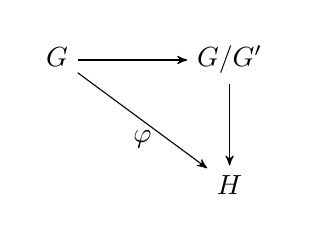
\begin{tikzpicture}
  \matrix (m)
    [
      matrix of math nodes,
      row sep    = 3em,
      column sep = 4em
    ]
    {
	    G & G / G' \\
	     & H            \\
    };
  \path
    (m-1-2) edge [->] node {} (m-2-2)
    (m-1-1.east |- m-1-2)
      edge [->] node {} (m-1-2)
      (m-1-1) edge [->] node [below] {$\varphi$} (m-2-2);
\end{tikzpicture}
\end{center}
	\end{itemize}
\end{prop}
The way to think about this is that by passing to the quotient by the commutator subgroup of \(G\), we collapse all commutators to identity. Hence, all elements in the quotient group commute. This is why we have such a strong property in that, if \(G' \leq H\), then \(G / H\) must be abelian.\\

One word of caution-- there can be elements of the commutator subgroup that \textit{cannot} be written as a single commutator \([x,y]\) for any \(x,y\). In other words, \(G'\) is not just the set of single commutators, but is the group generated by elements of that form.

\begin{prop}
	Let \(H,K \leq G\) be subgroups. The number of distinct ways of writing each element of the set \(HK\) in the form \(hk\), for some \(h \in H\), \(k \in K\), is \(\left| H \cap K \right| \).\\

	If \(H\cap K = 1\), then each element of \(HK\) can be written uniquely as a product \(hk\) for some \(h \in H\), \(k \in K\).
\end{prop}

\begin{thm}
	Let \(H,K\leq G\) be subgroups of \(G\) such that \(H,K \triangleleft G\) and \(H\cap K = 1\). Then
	\begin{align*}
		HK \cong H\times K
	\end{align*}
\end{thm}

\subsection{Free Groups}
\label{sub:free_groups}

The idea of the free group is to define a group \(F(S)\) to be generated by some set \(S\) with no relations on any of the elements of \(S\). For example, if \(S = \left\{ a,b \right\} \), then some elements of \(F(S)\) would be of the form \(a,aa,ab,abab,bab\), as well as the inverses of these elements. We call elements of a free group \textbf{words}. Then we can multiply elements in the free group simply by concatenation. Our goal will be to define this formally and show it indeed satisfies the necessary properties.

\begin{general}[Construction of Free Groups]
	Let \(S\) be a set, and let \(S^{-1}\) be a set disjoint from \(S\) such that there is a bijection from \(S\) to \(S^{-1}\). We denote the corresponding element for \(s \in S\) to be \(s\mapsto s^{-1}\in S^{-1}\), and furthermore we denote \((s^{-1})^{-1} = s\). Finally, we add a third singleton set disjoint from \(S,S^{-1}\) and call it \(\left\{ 1 \right\} \), and define it so \(1^{-1} = 1\). We also define that for any \(x \in S \cup S^{-1}\cup \left\{ 1 \right\} \), \(x^{1} = x\).\\

	A \textbf{word} on \(S\) is a sequence \((s_1,s_2,s_3,\ldots)\) where \(s_i \in S\cup S^{-1} \cup \left\{ 1 \right\} \), and \(s_i = 1\) for all \(i\geq N\) for some arbitrarily large \(N\) (so that words are "infinite", but not in practice). In order to get uniqueness of words, we say a word is \textbf{reduced} if
	\begin{align*}
		s_{i+1} \neq s_{i}^{-1} \quad \forall i, s_i \neq 1\\
		s_k = 1 \implies s_i = 1 \; \forall i \geq k
	\end{align*}
	We refer to the special word given by
	\begin{align*}
		(1,1,1,\ldots)
	\end{align*}
	to be the \textbf{empty word} and denote it by \(1\). Let \(F(S)\) be the set of reduced words on \(S\), and embed mKS into \(F(S)\) by
	\begin{align*}
		s \mapsto (s,1,1,1,\ldots)
	\end{align*}
	Hence we identify \(S\) with its image and consider \(S\subset F(S)\). Notie that if \(S = \emptyset\), \(F(S) = \left\{ 1 \right\} \).\\

	Now we simply introduce a binary operation on \(F(S)\), so that two words in \(F(S)\) are concatenated, then reduced to their reduced word form. We leave the details of defining this binary operation to the reader, but one can check that this operation is well-defined and satisfies all the properties of a group operation.
\end{general}

\begin{thm}
	\(F(S)\) is a group by the binary operation of word concatenation with reduction.
\end{thm}
Furthermore, free groups satisfy a special kind of universal property.
\begin{thm}
	Let \(G\) be a group, \(S\) a set, and \(\varphi :S\to G\) a set map. There is a unique group homomorphism \(\Phi :F(S) \to G\) such that the following diagram commutes:
\begin{center}
			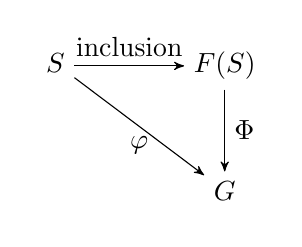
\begin{tikzpicture}
  \matrix (m)
    [
      matrix of math nodes,
      row sep    = 3em,
      column sep = 4em
    ]
    {
	    S & F(S) \\
	     & G            \\
    };
  \path
	  (m-1-2) edge [->] node [right] {\(\Phi \)} (m-2-2)
    (m-1-1.east |- m-1-2)
    edge [->] node [above] {inclusion} (m-1-2)
      (m-1-1) edge [->] node [below] {$\varphi$} (m-2-2);
\end{tikzpicture}
\end{center}

\end{thm}
This further shows that \(F(S)\) is unique up to a unique isomorphism, which is the identity map on the set \(S\).

\begin{defn}[Free Group]
	The group \(F(S)\) is called the \textbf{free group} on the set \(S\). A group \(F\) is a \textbf{free group} if there is some set \(S\) such that \(F = F(S)\), in which case we call \(S\) a set of \textbf{free generators} of \(F\). The cardinality of \(S\) is called the \textbf{rank} of the free group.
\end{defn}

\begin{thm}
	Subgroups of a free group are free.
\end{thm}
Furthermore, if \(G\leq F\) are free and \([F:G] = m\), then
\begin{align*}
	\textrm{rank}(G) = 1 + m(\textrm{rank}(F)-1)
\end{align*}
Proving this requires a lot of other tools, such as covering spaces.

\subsection{Presentations}
\label{sub:presentations}

Notice that if we take \(S = G\), then we can view \(G\) as a homomorphic image of the free group \(F(G)\) onto \(G\). Moreover, if \(G= \langle S \rangle \), there is a unique surjective homomorphism from  \(F(S)\) onto \(G\) which is the identity on \(S\). This allows us to construct a more powerful construction of presentations, generators, and relations.

\begin{defn}
	A subset \(S\subset G\) \textbf{generates \(G\)} by \(G = \langle S \rangle \) if and only if the map \(\pi :F(S) \to G\) which extends the identity map of \(S\) to \(G\) is surjective.
\end{defn}
This is distinct but equivalent to our earlier notion for subsets generating a group. However, it is more flexible, so we will use this from here on out.

\begin{defn}[Presentations, Generators, and Relations]
	Let \(S\subset G\) be a subset of \(G\) such that \(G = \langle S \rangle \). A \textbf{presentation} for \(G\) is a pair \((S,R)\), where \(R\) is a set of words in \(F(S)\) such that
	\begin{align*}
		\textrm{ncl}_{F(S)}(\langle R \rangle ) = \textrm{Ker}(\pi )
	\end{align*}
	where \(\textrm{ncl}\) denotes the normal closure (the smallest normal subgroup containing \(\langle R \rangle \)). The elements of \(S\) are called \textbf{generators}, and the elements of \(R\) are called \textbf{relations} of \(G\).\\

	We say \(G\) is \textbf{finitely generated} if there is a presentation \((S,R)\) such that \(S\) is finite. Furthermore, \(G\) is \textbf{finitely presented} if \(R\) is also finite.
\end{defn}
A word of caution-- the kernel of the map \(F(S) \to G\) is \textit{not} \(\langle R \rangle \), but instead the union of all subsets conjugate to \(\langle R \rangle \) (including \(\langle R \rangle \) itself). Furthermore, even if \(S\) is fixed, a group will have many different presentations.\\

Finally, often when writing relations, if we have \(w_1w_2^{-1} = 1\), we might instead write \(w_1=w_2\), or vice versa.

\subsection{Applying presentations to find homomorphisms and automorphisms}
\label{sub:applying_presentations_to_find_homomorphisms_and_automorphisms}

Suppose \(G\) is presented by \((\langle a,b \rangle , \langle r_1,\ldots,r_k \rangle )\). Then if \(a',b' \in H\) are elements that satisfy \(r_1,\ldots,r_k\), then there is a homomorphism from \(G\) into \(H\). If \(\pi :F(\left\{ a,b \right\} )\to G\) is the presentation homomorphism, we can define
\begin{align*}
	\pi ':F(\left\{ a,b \right\} ) \to H\\
	\pi'(a) = a', \; \pi'(b) = b'.
\end{align*}
This works because \(\textrm{Ker}\pi \leq \textrm{Ker}\pi'\), and so \(\pi '\) factors through \(\textrm{Ker}\pi \) and we get
\begin{align*}
	G \cong F(\left\{ a,b \right\} ) / \textrm{Ker}\pi \to H
\end{align*}
Moreover, if \(\langle a',b' \rangle = H = G\), then this homomorphism is an automorphism of \(G\)(!!). In the other direction, any automorphism on a presentation must send a set of generators to another set of generators satisfying the same relations.

\begin{exmp}[Dihedral presentation]
	Consider \(D_8 = \langle a,b \mid a^2 = b^{4} =1, aba = b^{-1} \rangle \). Any pair of elements \(a',b'\) that are of order 2 and 4 (and \(a'\) is noncentral) must satisfy the same relations. There are four noncentral elements of order 2, and two elements of order 4, so \(D_8\) has 8 automorphisms.
\end{exmp}
Similarly, any distinct pair of elements of order \(4\) in \(Q_8\) that are not inverses of each other necessarily generate \(Q_8\) and satisfy its relations. There are \(24\) such pairs, so \(\left| \textrm{Aut}(Q_8) \right| =24\). As one can see, free groups are an incredibly useful tool to classify these maps.

% \printindex
\end{document}


\chapter{Sylow and Structure Theorems}
\label{cha:sylow_and_structure_theorems}

\documentclass{memoir}
\usepackage{notestemplate}

% \begin{figure}[ht]
%     \centering
%     \incfig{riemmans-theorem}
%     \caption{Riemmans theorem}
%     \label{fig:riemmans-theorem}
% \end{figure}

\begin{document}

\begin{defn}
	Let \(G\) be a group and \(p\) prime. If \(\left| G \right| = p^{\alpha }\) for \(\alpha \geq 1\) then \(G\) is called a \textbf{\(p\)-group}. Even if \(G\) has different order, if a subgroup has order \(p^{\alpha }\), then we call the subgroups \textbf{\(p\)-subgroups}.\\

	In the specific case where \(\left| G \right| = p^{\alpha }m\) for \(p \not\mid m\), then a subgroup of \(G\) of order \(p^{\alpha }\) is called a \textbf{Sylow \(p\)-subgroup of \(G\)}.
\end{defn}
We denote the set of Sylow \(p\)-subgroups of \(G\) by \(\textrm{Syl}_p(G)\), and the number of Sylow \(p\)-subgroups of \(G\) by \(n_p(G)\).

\begin{thm}[Sylow's Theorem]
	Let \(G\) be a group of order \(n = p^{a}m\), where \(p\) is prime and \(p \not\mid m\). Then
	\begin{itemize}
		\item G contains a Sylow \(p\)-subgroup.
		\item The number of Sylow \(p\)-subgroups of order \(p^{a}\) is congruent to \(1 \pmod p\) and all these subgroups are conjugate. Furthermore, \(n_p\mid m\) as \(n_p\) is the index in \(G\) of the normalizer of any Sylow \(p\)-subgroup.
		\item Any \(p\)-subgroup is a subgroup of a Sylow \(p\)-subgroup.
	\end{itemize}
\end{thm}
Moreover, Sylow \(p\)-subgroups are not only conjugate, but isomorphic.

\begin{cor}
	Let \(P\) be a Sylow \(p\)-subgroup of \(G\). The following are equivalent:
	\begin{itemize}
		\item \(P\) is the unique Sylow \(p\)-subgroup of \(G\) ; \(n_p = 1\) 
		\item \(P \triangleleft G\)
		\item \(P \textrm{char}G\) 
		\item If \(X\subset G\) such that \(\left| x \right| = p^{k_x}\)for all \(x \in X\), then \(\langle X \rangle \) is a \(p\)-group.
	\end{itemize}
\end{cor}

\begin{exmp}
	Let \(G\) be finite and \(p\) prime.
	\begin{itemize}
		\item If \(p \not\mid \left| G \right| \), the Sylow \(p\)-subgroup of \(G\) is trivial. If \(\left| G \right| = p^{\alpha }\), then \(G\) is the unique Sylow \(p\)-subgroup of \(G\).
		\item A finite abelian group has a unique Sylow \(p\)-subgroup for each prime \(p\) called the \textbf{\(p\)-primary component} of the abelian group. It consists of all elements \(g\) such that \(\left| g \right| = p^{k_g}\).
		\item \(S_3\) has three Sylow 2-subgroups:
			\begin{align*}
				\langle (12) \rangle , \langle (23) \rangle , \langle (13) \rangle .
			\end{align*}
			It has a unique (hence normal) Sylow 3-subgroup \(\langle (123) \rangle = A_3\).
		\item \(A_4\) has a unique Sylow 2-subgroup \(\langle (12)(34),(13)(24) \rangle \cong V_4\). It has four Sylow 3-subgroups:
			\begin{align*}
				\langle (123) \rangle , \langle (124) \rangle , \langle (134) \rangle , \langle (234) \rangle .
			\end{align*}
		\item \(S_4\) has  \(n_2 = 3\) and \(n_3 = 4\). Furthermore, \(S_4\) has a subgroup isomorphic to \(D_{8}\), and hence by conjugacy properties every \(2\)-subgroup of \(S_4\) is isomorphic to \(D_8\).
	\end{itemize}
\end{exmp}

Sylow's theorem is incredibly useful for showing that groups of a particular order cannot be simple. For example, it can be used to show that if a group is of order 60 and has more than one Sylow 5-subgroup, it must be simple, and hence proves easier that \(A_5\) is simple (and its uniqueness as a simple group of order 60).\\

Before we get into some nice applications of Sylow's theorem, we will construct some properties for \(p\)-groups that will be useful later.

\begin{defn}[Maximal Subgroup]
	A \textbf{maximal subgroup} of a group \(G\) is a proper subgroup \(M<G\) such that there ar eno subgroups \(H<G\) that satisfy
	\begin{align*}
		M < H < G.
	\end{align*}
\end{defn}
We can easily see that every proper subgroup of a finite group is contained in a maximal subgroup, but infinite groups need not have maximal subgroups.

\begin{thm}[Properties of \(p\)-groups]
	Let \(p\) be a prime and let \(P\) be a group of order \(p^{a}\) for \(a\geq 1\). Then
	\begin{itemize}
		\item \(Z(P) \neq 1\) 
		\item If \(H \triangleleft P\) is nontrivial, then \(H\cap Z(P) \neq 1\). Furthermore, every normal subgroup of order \(p\) is contained in \(Z(P)\).
		\item If \(H \triangleleft P\) then \(H\) contains a subgroup \(H'\) of order \(p^{b}\) so that \(H' \triangleleft P\) for each divisor \(p^{b}\mid \left| H \right| \).
		\item If \(H<P\) then \(H< N_P(H)\) (every proper subgroup of \(P\) is a proper subgroup of its normalizer in \(P\))
		\item Every maximal subgroup \(M<P\) is of index \(p\) and \(M \triangleleft P\).
	\end{itemize}
\end{thm}

\begin{thm}[Cauchy's Theorem]
	If a prime number \(p\) divides the order of a group \(G\), then \(G\) contains an element of order \(p\).
\end{thm}
A group of \(p\)-power order, acting on a set of size divisible by \(p\), has the property that the number of fixed points is divisible by \(p\). Hence, if there is at least one fixed point, then there are at least \(p\).

\begin{thm}
	Let \(G\) be a group of order \(p^{a}m\), where \(p\) is prime not dividing \(m\). Then, for \(0\leq i\leq a\),
	\begin{itemize}
		\item \(G\) contains a subgroup of order \(p^{i}\) 
		\item if \(i<m\), then any subgroup of order \(p^{i}\) is contained normally in a subgroup of order \(p^{i+1}\).
	\end{itemize}
\end{thm}

\begin{thm}
	The center of a non-trivial \(p\)-group is non-trivial. Furthermore, if \(\left| P \right| = p^{a}\), then \(P\) has a chain
	\begin{align*}
		P_0<P_1<\ldots<P_a=P
	\end{align*}
	of subgroups, where \(\left| P_i \right| =p^{i}\) and each is a normal subgroup of \(P\). Moreover, \(P_{i+1} / P_i \cong C_p\).
\end{thm}

\end{document}

\documentclass{memoir}
\usepackage{notestemplate}

%\logo{~/School-Work/Auxiliary-Files/resources/png/logo.png}
%\institute{Rice University}
%\faculty{Faculty of Whatever Sciences}
%\department{Department of Mathematics}
%\title{Class Notes}
%\subtitle{Based on MATH xxx}
%\author{\textit{Author}\\Gabriel \textsc{Gress}}
%\supervisor{Linus \textsc{Torvalds}}
%\context{Well, I was bored...}
%\date{\today}

%\makeindex

\begin{document}

% \maketitle

% Notes taken on 

\section{Characterization of Finitely Generated Groups}
\label{sec:characterization_of_finitely_generated_groups}
(Note: One can read this section without having seen Sylow's theorem and simply ignore any statement about Sylow \(p\)-groups. However, the content here should be revisited once the reader encounters Sylow's theorem elsewhere)\\

We have already begun classifying groups via Sylow's theorem, but once we utilize the tools of direct products, we can more generally classify groups. Hence the theorems in this section are an extension of the tools given via Sylow's theorem.\\

A group \(G\) is \textbf{finitely generated} if there is a finite subset \(A\subset G\) such that \(G = \langle A \rangle \).

\begin{defn}[Free Abelian Group]
	Let \(r \in \N\) be given. We define the \textbf{free abelian group of rank \(r\)} to be the group
	\begin{align*}
		\Z^{r} = \Z\times \Z\times \ldots^{r}\times \Z.
	\end{align*}
	If \(r = 0\), then \(\Z^{0}=1\).
\end{defn}

\begin{thm}[Fundamental Theorem of Finitely Generated Abelian Groups]
	Let \(G\) be a finitely generated abelian group. Then
	\begin{align*}
		G \cong \Z^{r} \times \Z_{n_1} \times \Z_{n_2}\times \ldots\times \Z_{n_s}
	\end{align*}
	for some integers \(r,n_1,n_2,\ldots,n_s\) such that \(r\geq 0\), \(n_i \geq 2\), and \(n_{i+1}\mid n_i\). Furthermore, this factorization of \(G\) is unique.\\

	We call \(r\) the \textbf{free rank} or \textbf{Betti number} of \(G\), and the integers \(n_1,n_2,\ldots,n_s\) the \textbf{invariant factors of \(G\)}. The factorization above is hence referred to as the \textbf{invariant factor decomposition of \(G\).}
\end{thm}
A finitely generated abelian group is a finite group if and only if its free rank is zero. Furthermore, if  \(G\) is a finite abelian group, then its order is the product of its invariant factors, and we say that \(G\) is of \textbf{type  \((n_1,\ldots,n_s)\)}.\\

Observe that because \(n_1\) is the largest invariant factor, and each \(n_i\mid n\), if \(p\) is a prime divisor of \(\left| G \right| =n\), then \(p \mid n_1\).

\begin{cor}
	If \(n\) is the product of distinct primes, then up to isomorphism the only abelian group of order \(n\) is \(\Z_n\).
\end{cor}

The fact that \(n_{i+1} \mid n_i\) really puts a strong restriction on the structure of finite abelian groups. When \(n\) is finite, we will see that the types of abelian groups of order \(n\) correspond to the factorization of \(n\).

\begin{thm}[Primary Decomposition Theorem for Finite Abelian Groups]
	Let \(G\) be an abelian group with \(\left| G \right| =n >1\), and let the unique factorization of \(n\) into distinct prime powers be given by
	\begin{align*}
		n = p^{\alpha_1}_1 p_2^{\alpha_2}\ldots p_k^{\alpha_k}.
	\end{align*}
	Then
	\begin{align*}
		G \cong A_1\times A_2 \times \ldots\times A_k
	\end{align*}
	where \(\left| A_i \right| = p_i^{\alpha_i}\), and
	\begin{align*}
		A_i \cong \Z_{p_i^{\beta_1}}\times \Z_{p_i^{\beta_2}}\times \ldots\times \Z_{p_i^{\beta_t}}
	\end{align*}
	where
	\begin{align*}
		\beta_1 + \beta_2 + \ldots + \beta_t = \alpha_i \\
		\beta_1\geq \beta_2\geq \ldots\geq \beta_t \geq 1.
	\end{align*}
	Furthermore, this decomposition is unique.\\

	We call the integers \(p_i^{\beta_j}\) the \textbf{elementary divisors of \(G\)}. Thhis decomposition is called the \textbf{elementary divisor decomposition of \(G\)}.
\end{thm}
The subgroups \(A_i\) are the Sylow \(p_i\)-subgroups of \(G\), and hence the theorem essentially states that \(G\) is isomorphic to the direct product of its Sylow subgroups (which are normal and hence unique, because \(G\) is abelian). \\

Notice that the decomposition in \(A\) is the invariant factor decomposition of \(A\) with the divisibility condition in the fundamental theorem of finitely generated abelian groups, and hence the elementary divisors of \(G\) are the invariant factors of the Sylow \(p_i\)-subgroups.\\

The advantage of this representation is that it lets us easier determine all possible abelian groups of a certain order. Because the \(\beta_i\) are all uniquely determined and satisfy the above properties, it forms a partition of  \(\alpha  \), and hence we simply look at all combinations of partitions of \(\alpha_i\).

\begin{exmp}[Abelian groups of order \(p^5\)]
	Consider an abelian group \(G\) with \(\left| G \right| = p^{5}\) for some \(p\) prime. Then this technique allows us to distinguish all unique groups like so:
	\begin{align*}
		\begin{array}{c | c}
		\textbf{Invariant Factors} & \textbf{Abelian Groups}\\
			\hline
		5 &\quad \Z_{p^{5}}\\
		4,1 &\quad \Z_{p^{4}}\times \Z_p\\
		3,2 &\quad \Z_{p^3}\times \Z_{p^2}\\
		3,1,1 &\quad \Z_{p^3}\times \Z_p \times \Z_p\\
		2,2,1 &\quad \Z_{p^2}\times \Z_{p^2}\times \Z_p\\
		2,1,1,1 &\quad \Z_{p^2}\times \Z_p\times \Z_p\times \Z_p\\
		1,1,1,1,1 &\quad \Z_p\times \Z_p \times \Z_p \times \Z_p \times \Z_p
		\end{array}
	\end{align*}
	Hence, there are exactly 7 distinct (up to isomorphism) groups of order \(p^{5}\).
\end{exmp}

Of course, it would be more helpful if we had a nice way to pass between the two representations of a factorization of a finite abelian group\ldots
\begin{prop}
	Let \(m,n \in \Z_+\). Then \(\Z_{m}\times \Z_n \cong \Z_{mn}\) if and only if \((m,n) = 1\).\\

	If \(n = p_1^{\alpha_1}p_2^{\alpha_2}\ldots p_k^{\alpha_k}\), then
	\begin{align*}
		\Z_n \cong \Z_{p_1}^{\alpha_1}\times \Z_{p_2^{\alpha_2}} \times  \ldots \times \Z_{p_k^{\alpha_k}}.
	\end{align*}
\end{prop}

Then we can go back and forth between the two representations by: factoring out our \(n_i\)'s into their prime decomposition, in which case collecting each \(p_j\) factor gives you each of the Sylow \(p_j\) subgroups.\\

For the reverse direction, we group the elementary divisors by their \(p_i\) value, then take the product across different \(p_i\) in decreasing order. For example, if the elementary divisors of \(G\) are \(2,3,2,25,3,2\), then \(\left| G \right| = 2^3\cdot 3^2\cdot 5^2\), so the invariant factors of \(G\) are \((2_1^{1}\cdot 3_1^{1}\cdot 5^2_1)\), \((2_2^{1}\cdot 3_2^{1}\cdot 5_2^{0})\), and \((2_3^{1}\cdot 3_3^{0}\cdot 5_3^{0})\), so that
\begin{align*}
	G \cong \Z_{150} \times \Z_6 \times \Z_2.
\end{align*}
This makes it very easy to compare groups of the same order, because if their elementary divisors differ, they cannot be isomorphic.

\begin{defn}[Rank]
	If \(G\) is a finite abelian group of type \((n_1,\ldots,n_t)\), the integer \(t\) is called the \textbf{rank} of \(G\).
\end{defn}

\begin{prop}
	\begin{itemize}
		\item If \(\left| G \right| = p\), then \(G \cong Z_p\)
		\item If \(\left| G \right| =p^2\), then \(G\) is Abelian and \(G \cong Z_{p^2} \text{ OR }Z_p \times Z_p\)
		\item Let \(p>2\), if \(\left| G \right| = 2p\), then \(G \cong Z_{2p} \text{ OR } D_p\).
	\end{itemize}
\end{prop}

The first two we have already seen from automorphisms. We will see the latter one after developing more group theory.

% \printindex

\end{document}


\chapter{Chain Conditions and Sequences}
\label{cha:chain_conditions_and_sequences}



\documentclass{memoir}
\usepackage{notestemplate}

%\logo{~/School-Work/Auxiliary-Files/resources/png/logo.png}
%\institute{Rice University}
%\faculty{Faculty of Whatever Sciences}
%\department{Department of Mathematics}
%\title{Class Notes}
%\subtitle{Based on MATH xxx}
%\author{\textit{Author}\\Gabriel \textsc{Gress}}
%\supervisor{Linus \textsc{Torvalds}}
%\context{Well, I was bored...}
%\date{\today}

%\makeindex

\begin{document}

% \maketitle

% Notes taken on 06/03/21

\section{Nilpotent and Solvable Groups}
\label{sec:nilpotent_and_solvable_groups}

\begin{defn}[Nilpotence]
	For any group \(G\), define the following subgroups inductively:
	\begin{align*}
		Z_0(G) = 1, \quad Z_1(G) = Z(G),\\
		Z_i(G) \subset Z_{i+1}(G) < G \quad Z_{i+1}(G) / Z_i(G) = Z(G / Z_i(G))
	\end{align*}
	That is, \(Z_{i+1}(G)\) is a subgroup of \(G\) containing \(Z_i(G)\) that is the complete preimage in \(G\) of the center of \(G / Z_i(G)\) under the natural projection. We call the chain of subgroups
	\begin{align*}
		Z_0(G) \leq Z_1(G) \leq Z_2(G) \leq \ldots
	\end{align*}
	the \textbf{upper central series} of \(G\).\\

	A group \(G\) is called \textbf{nilpotent} if \(Z_c(G) = G\) for some \(c \in \Z\); the smallest such \(c\) is called the \textbf{nilpotence class of \(G\)}.
\end{defn}
Nilpotence is a more general form of being abelian-- a group may not be abelian, but when one quotients out abelian elements, the quotient might have abelian elements within itself-- if we can iterate this process until all elements are abelian under some quotient of centers, then our group is nilpotent.

\begin{rmrk}
	If \(G\) is abelian, then \(G\) is nilpotent with nilpotence class \(1\). This holds because \(Z(G) = G\). Furthermore, we will show the following hierarchy:
	\begin{align*}
		\text{cyclic groups}\subset \text{abelian groups}\subset \text{nilpotent groups}\subset \text{solvable groups}\subset \text{all groups}
	\end{align*}
	If \(G\) is finite, there must be an integer \(N\) so that for all \(n\geq N\),
	\begin{align*}
		Z_n(G) = Z_{n+1}(G) = \ldots
	\end{align*}
	If there is a point such that \(Z_n(G) = Z_{n+1}(G)\), then the upper limit has been reached.\\

	Infinite groups act a little bit differently with nilpotency; for example, \(Z_i(G) < G\) might all be proper subgroups of \(G\) (i.e \(G\) is not nilpotent), yet
	\begin{align*}
		G = \bigcup_{i=0} ^{\infty}Z_i(G).
	\end{align*}
	We call these groups \textbf{hypernilpotent}.
\end{rmrk}
\begin{prop}
	Let \(p\) be a prime and let \(P\) be a group of order \(p^{a}\). Then \(P\) is nilpotent of nilpotence class at most \(a-1\).
\end{prop}
\begin{proof}
	Observe that for \(i\geq 0\), \(P / Z_i(P)\) is a \(p\)-group. Hence, if \(\left| P / Z_i(P) \right| >1\), then \(Z(P / Z_i(P)) \neq 1\).\\

	Assume that \(Z_i(P) \neq G\). Then 
	\begin{align*}
	\left| Z_{i+1}(P)  \right| \geq p \left| Z_i(P) \right| 
	\end{align*}
	and so \(\left| Z_{i+1}(P) \right| \geq p^{i+1}\). Thus, 
\begin{align*}
\left| Z_a(P) \right| \geq p^{a} \implies P = Z_a(P)
\end{align*}
	This is just an upper bound however-- \(P\) is only nilpotence of class \(a\) if \(\left| Z_i(P) \right| = p^{i}\). This cannot occur, however, as \(Z_{a-2}(P)\) would have index \(p^2\) in \(P\), and hence be abelian (in which case \(Z_{a-1}(P) = P\)). Hence, the class of \(P\) is at most \(a-1\).
\end{proof}

\begin{exmp}
	Both \(D_8\) and \(Q_8\) are nilpotent of class \(2\). Moreover, \(D_{2^{n}}\) is nilpotent of class \(n-1\). This can be proven inductively by showing \(\left| Z(D_{2^{n}}) \right| =2\) and \(D_{2^{n}}/ Z(D_{2^{n}}) \cong D_{2^{n-1}}\) for \(n\geq 3\).\\

	If \(n\) is not a power of 2, then \(D_{2n}\) is not nilpotent.
\end{exmp}

\begin{thm}
	Let \(G\) be a finite group, and let \(p_1,p_2,\ldots,p_s\mid \left| G \right| \) be distinct primes that divide its order. Let \(P_i \in \textrm{Syl}_{p_i}(G)\). The following are equivalent:
	\begin{itemize}
		\item \(G\) is nilpotent
		\item if \(H<G\), then \(H <  N_G(H)\)
		\item \(P_i \triangleleft G\) for all \(1\leq i\leq s\) 
		\item \(G \cong P_1\times P_2\times \ldots\times P_s\)
	\end{itemize}
\end{thm}
This theorem proves part of the fundamental theorem of finite abelian groups.

\begin{cor}
	A finite abelian group is the direct product of its Sylow subgroups.
\end{cor}

\begin{prop}
	If \(G\) is a finite group such that, for all \(n\mid \left| G \right| \) positive, \(G\) has at most \(n\) elements that satisfy \(x^{n}=1\), then \(G\) is cyclic.
\end{prop}
\begin{prop}[Frattini's Argument]
	Let \(G\) be a finite group and \(H \triangleleft G\), and let \(P\) be a Sylow \(p\)-subgroup of \(H\). Then
	\begin{align*}
		G = HN_G(P)\\
		\left| G : H \right| \mid \left| N_G(P) \right| .
	\end{align*}
\end{prop}

\begin{prop}
	A finite group is nilpotent if and only if every maximal subgroup is normal.
\end{prop}
\begin{proof}
	Let \(G\) be a finite nilpotent group and let \(M\) be the maximal subgroup of \(G\). Because \(M < N_G(M)\), by maximality, \(N_G(M) = G\) and hence \(M \triangleleft G\).\\

	For the reverse direction, assume every maximal subgroup of the finite group \(G\) is normal. Let \(P\) be a Sylow \(p\)-subgroup of \(G\). For the sake of contradiction, assume that \(P \not\triangleleft G\), and let \(M\) be a maximal subgroup of \(G\) containing \(N_G(P)\). Frattini's argument tells us that \(G = MN_G(P)\). But \(N_G(P) \leq M\) and so \(MN_G(P) = M\) giving us a contradiction. Hence \(P \triangleleft G\) which is equivalent to nilpotency.
\end{proof}

\begin{defn}[Lower central series]
	Let \(G\) be a group, and define the following subgroups inductively:
	\begin{align*}
		G^{0} = G, \quad G^{1}= [G,G],\\
		G^{i+1}= [G,G^{i}].
	\end{align*}
	Then the chain of groups
	\begin{align*}
		G^{0}\geq G^{1}\geq G^2\geq \ldots
	\end{align*}
	is called the \textbf{lower central series} of \(G\).
\end{defn}
\begin{hw}
	Prove that \(G^{i}\) is a characteristic subgroup of \(G\) for all \(i\).
\end{hw}

\begin{thm}
	A group \(G\) is nilpotent of class \(c\) if and only if \(c\) is the smallest nonnegative integer such that \(G^{c}=1\). If \(G\) is nilpotent of class \(c\) then
	\begin{align*}
		Z_i(G) \leq G^{c-i-1}\leq Z_{i+1}(G) \quad \forall i \in \left\{ 0,1,\ldots,c-1 \right\} .
	\end{align*}
\end{thm}
The terms in the upper and lower central series do not necessarily coincide (although this does happen sometimes).

\begin{rmrk}
	If \(G\) is abelian, then \(G' = G^{1} = 1\) and so the lower central series is identity after one term. Similar to the upper central series, for any finite group there is some integer \(N\) so that for all \(n\geq N\),
	\begin{align*}
		G^{n}= G^{n+1} = G^{n+2} = \ldots
	\end{align*}
	For non-nilpotent groups, \(G^{n}\) is a nontrivial subgroup of \(G\). Once equality holds for some \(G^{n}= G^{n+1}\), it holds for all terms after.
\end{rmrk}

\begin{thm}[Krull-Schmidt Theorem]
	We say that a group \(G\) satisfies the \textbf{ascending chain condition} on subgroups if every sequence of subgroups of \(G\)
	\begin{align*}
		1 = G_0\leq G_1\leq G_2\leq \ldots
	\end{align*}
	is eventually constant. Likewise, we say that \(G\) satisfies the \textbf{descending chain condition} on subgroups if
	\begin{align*}
		G = G_0 \geq G_1 \geq G_2 \geq \ldots
	\end{align*}
	is eventually constant.\\

	Assume \(G\) is a group that satisfies one of these chain conditions on normal subgroups. Then there is a unique way to write \(G\) by
	\begin{align*}
		G \cong G_1 \times G_2 \times \ldots\times G_k
	\end{align*}
	where \(G_k\) are indecomposable (i.e. cannot be written as a direct product of two proper subgroups).
\end{thm}
Note that the decomposition could be non-trivial-- all the theorem gives is uniqueness.
\subsection{Solvable Groups}
\label{sub:solvable_groups}

\begin{defn}
	Let \(G\) be a group. A \textbf{subnormal series} is a sequence of subgroups satisfying:
	\begin{align*}
		1 = H_0 \triangleleft H_1 \triangleleft \ldots \triangleleft H_s = G
	\end{align*}
	If moreover \(H_i \triangleleft G\) for all \(i\), then we say it is a \textbf{normal series}.\\

	A \textbf{solvable group} is a group with a subnormal series such that  \(H_{i+1} / H_i\) is abelian.
\end{defn}
We will see that in fact the subnormal series of a solvable group is actually a normal series.


We will shortly see that this is related to the notions described above.

\begin{defn}
	Let \(G\) be a group. We define the following sequence of subgroups inductively:
	\begin{align*}
		G^{(0)}= G, \quad G^{(1)} = [G,G]\\
		G^{(i+1)}= [G^{(i)}, G^{(i)}]
	\end{align*}
	This series of subgroups is called the \textbf{derived} or \textbf{commutator} series of \(G\).
\end{defn}
Note that sometimes we notate \(G^{(1)}= G'\), \(G^{(2)} = G''\), and so on. One can show that \(G^{(i)}\) is characteristic in \(G\).\\

Caution must be used here-- \(G^{(0)} = G^{0}\), \(G^{(1)}= G^{1}\), but this does not hold necessarily for all \(i\). The terms are noticably smaller, so \(G^{(i)}\leq G^{i}\).

\begin{thm}
	A group \(G\) is solvable if and only if \(G^{(n)}=1\) for some \(n\geq 0\).\\

	If \(G\) is solvable, the smallest nonnegative \(n\) for which \(G^{(n)}=1\) is called the \textbf{solvable length} of \(G\).
\end{thm}

\begin{prop}
	Let \(G, K\) be groups, let \(H\leq G\), and let \(\varphi :G\to K\) be a surjective homomorphism. Then
	\begin{itemize}
		\item \(H^{(i)}\leq G^{(i)}\)-- thus if \(G\) is solvable, then \(H\) is solvable
		\item \(\varphi (G^{(i)} = K^{(i)}\)-- homomorphic images and quotient groups of solvable groups are solvable
		\item If \(N \triangleleft G\) and \(N\), \(G / N\) are solvable, then so is \(G\).
	\end{itemize}
\end{prop}

\begin{thm}
	Let \(G\) be a finite group.
	\begin{itemize}
		\item If \(\left| G \right| = p^{a}q^{b}\) for some primes \(p,q\), then \(G\) is solvable (Burnside)\\
		\item If for every prime \(p \mid \left| G \right| \) we factor the order of \(G\) as \(\left| G \right| = p^{a}m\) where \((p,m) = 1\), and \(G\) has a subgroup of order \(m\), then \(G\) is solvable (Philip Hall)
		\item If \(\left| G \right| \) is odd then \(G\) is solvable (Feit-Thompson)
		\item If for every pair of elements \(x,y \in G\), \(\langle x,y \rangle \) is a solvable group, then \(G\) is solvable.
	\end{itemize}
\end{thm}


% \printindex
\end{document}

\documentclass{memoir}
\usepackage{notestemplate}

\usetikzlibrary{arrows,chains,matrix,positioning,scopes}

\makeatletter
\tikzset{join/.code=\tikzset{after node path={%
\ifx\tikzchainprevious\pgfutil@empty\else(\tikzchainprevious)%
edge[every join]#1(\tikzchaincurrent)\fi}}}
\makeatother

\tikzset{>=stealth',every on chain/.append style={join},
every join/.style={->}}
%\logo{~/School-Work/Auxiliary-Files/resources/png/logo.png}
%\institute{Rice University}
%\faculty{Faculty of Whatever Sciences}
%\department{Department of Mathematics}
%\title{Class Notes}
%\subtitle{Based on MATH xxx}
%\author{\textit{Author}\\Gabriel \textsc{Gress}}
%\supervisor{Linus \textsc{Torvalds}}
%\context{Well, I was bored...}
%\date{\today}

%\makeindex

\begin{document}

% \maketitle

% Notes taken on 

Let \(A\) and \(C\) be arbitrary groups.. One question worth exploring is if there exists a group \(B\) such that \(A / B \cong C\)-- that is, \(B\) is an extension of \(C\) by \(A\). The tools we develop to understand this question are exact sequences. If \(A\) is isomorphic to a subgroup of \(B \), there is an injective homomorphism from \(A\) to \(B\). And if \(C\) is isomorphic to the quotient, then there is a surjective homomorphism from \(B\) to \(C\). This will give us a chain
\begin{align*}
	A \to B \to C
\end{align*}
where the homomorphisms are compatible with. We formalize this idea via exact sequences.

\begin{defn}[Exact Sequences]
	Let \(\alpha ,\beta \) be homomorphisms so that
	\begin{align*}
		X \to^{\alpha } Y \to^{\beta }Z.
	\end{align*}
	If \(\textrm{Im}(\alpha ) = \textrm{Ker}(\beta )\), then we say the pair of homomorphisms are \textbf{exact}.\\

	A sequence of homomorphisms
	\begin{align*}
		\ldots \to X_{n-1} \to X_n \to X_{n+1} \to \ldots
	\end{align*}
	is said to be an \textbf{exact sequence} if it is exact at every \(X_n\) between a pair of homomorphisms.
\end{defn}
Hence, our goal is to see whether we can form an exact sequence \(A\to B\to C\). Our notions of injectivity and surjectivity correspond exactly to the notions of exactness.
\begin{prop}
	Let \(A,B,C\) be groups. Then the sequence
	\begin{align*}
		0 \to A \to^{\psi }B
	\end{align*}
	is exact at \(A\) if and only if \(\psi \) is injective. Likewise, the sequence
	\begin{align*}
		B \to^{\varphi }\to C \to 0
	\end{align*}
	is exact at \(C\) if and only if \(\varphi \) is surjective.
\end{prop}
Combining the two ideas, the sequence
\begin{align*}
	0 \to A \to^{\psi }B \to^{\varphi }C \to 0
\end{align*}
is exact if and only if \(\psi \) is injective, \(\varphi \) is surjective, and \(\textrm{Im}(\psi ) = \textrm{Ker}(\varphi )\).

\begin{defn}
	An exact sequence of the form
	\begin{align*}
		0 \to A \to^{\psi }B \to^{\varphi }C \to 0
	\end{align*}
	is called an \textbf{short exact sequence}.
\end{defn}
Our goal then is to determine if two groups admit a short exact sequence, and if so, how many.\\

Notice that any exact sequence can be written as a succession of short exact sequences. For example, if
\begin{align*}
	X \to^{\alpha }Y \to^{\beta }Z
\end{align*}
is exact at \(Y\), then equivalently
\begin{align*}
	0 \to \alpha (X) \to Y \to Y / \textrm{Ker}(\beta ) \to 0
\end{align*}
is a short exact sequence.

\begin{exmp}
	
\end{exmp}

For fixed \(A,C\), there can be many extensions of \(C\) by  \(A\). Hence, we need to determine a notion of a homomorphism to distinguish exact sequences.

\begin{defn}[Homomorphism of Short Exact Sequences]
	Let
	\begin{align*}
		0 \to A \to B \to C \to 0\\
		0 \to A' \to B' \to C' \to 0
	\end{align*}
	be two short exact sequences of groups. A \textbf{homomorphism of short exact sequences} is a collection of group homomorphisms \(\alpha ,\beta ,\gamma \) such that the following diagram commutes:
\begin{center}
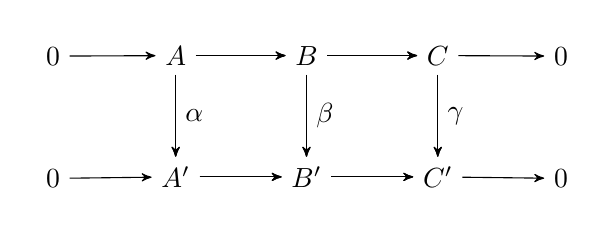
\begin{tikzpicture}
  \matrix (m) [matrix of math nodes, row sep=3em, column sep=3em]
    { 0 & A  & B  & C  & 0 \\
      0 & A' & B' & C' & 0 \\ };
  { [start chain] \chainin (m-1-1);
    \chainin (m-1-2);
    { [start branch=A] \chainin (m-2-2)
        [join={node[right] {$\alpha $}}];}
    \chainin (m-1-3) [join={node[above] {}}];
    { [start branch=B] \chainin (m-2-3)
        [join={node[right] {$\beta $}}];}
    \chainin (m-1-4) [join={node[above] {}}];
    { [start branch=C] \chainin (m-2-4)
        [join={node[right] {$\gamma $}}];}
    \chainin (m-1-5); }
  { [start chain] \chainin (m-2-1);
    \chainin (m-2-2);
    \chainin (m-2-3) [join={node[above] {}}];
    \chainin (m-2-4) [join={node[above] {}}];
    \chainin (m-2-5); }
\end{tikzpicture}
\end{center}
This is an \textbf{isomorphism of short exact sequences} if \(\alpha ,\beta ,\gamma \) are isomorphisms in which case the extensions \(B,B'\) are \textbf{isomorphic extensions}.\\

The two exact sequences are called \textbf{equivalent} if \(A = A'\), \(C = C'\), and there is an isomorphism between them where  \(\alpha ,\gamma \) are identity. In this case \(B\) and \(B'\) are \textbf{equivalent extensions}.
\end{defn}
Equivalency by extensions is strongesomorphisms between \(B\) and \(B'\)-- it tells us that there is an isomorphism between \(B\) and \(B'\) that restricts to an isomorphism from \(A\) to \(A'\) and induces an isomorphism on the quotients by \(C\) and \(C'\).

\begin{exmp}
	
\end{exmp}

\begin{prop}[Short Five Lemma]
	Let \(\alpha ,\beta ,\gamma \) be a homomorphism of short exact sequences
\begin{center}
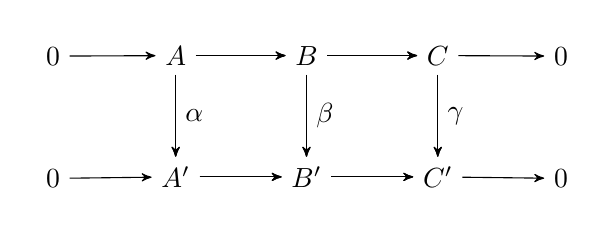
\begin{tikzpicture}
  \matrix (m) [matrix of math nodes, row sep=3em, column sep=3em]
    { 0 & A  & B  & C  & 0 \\
      0 & A' & B' & C' & 0 \\ };
  { [start chain] \chainin (m-1-1);
    \chainin (m-1-2);
    { [start branch=A] \chainin (m-2-2)
        [join={node[right] {$\alpha $}}];}
    \chainin (m-1-3) [join={node[above] {}}];
    { [start branch=B] \chainin (m-2-3)
        [join={node[right] {$\beta $}}];}
    \chainin (m-1-4) [join={node[above] {}}];
    { [start branch=C] \chainin (m-2-4)
        [join={node[right] {$\gamma $}}];}
    \chainin (m-1-5); }
  { [start chain] \chainin (m-2-1);
    \chainin (m-2-2);
    \chainin (m-2-3) [join={node[above] {}}];
    \chainin (m-2-4) [join={node[above] {}}];
    \chainin (m-2-5); }
\end{tikzpicture}
\end{center}
\begin{itemize}
	\item If \(\alpha ,\gamma \) are injective then so is \(\beta \) 
	\item If \(\alpha ,\gamma \) are surjective then so is \(\beta \) 
	\item If \(\alpha ,\gamma \) are isomorphisms then so is \(\beta \)
\end{itemize}
\end{prop}

\begin{proof}[Proof of Short Five Lemma]
	
\end{proof}
There is always at least one extension of a group \(C\) by \(A\) given by \(B = A \rtimes C\).

\begin{defn}
	If
	\begin{align*}
		1 \to A \to^{\psi }B \to^{\varphi }C \to 1
	\end{align*}
	is a short exact sequence of groups, then the sequence is \textbf{split} if there is a sugroup complement to \(\psi (A)\) in \(B\). Then up to isomorphism \(B = A \rtimes C\) up to isomorphism by
	\begin{align*}
		B = \psi (A) \rtimes C'
	\end{align*}
	for some subgroup \(C'\), which satisfies \(\varphi (C') \cong C\).\\

	We say \(B\) is a \textbf{split extension of \(C\) by \(A\)}.
\end{defn}
This is really just the question of existence of a complement to \(\psi (A)\) in \(B\) that is isomorphic by \(\varphi \) to \(C\).

\begin{prop}
	The short exact sequence of groups
	\begin{align*}
		1 \to A \to^{\psi }B \to^{\varphi }C \to 0
	\end{align*}
	of groups is split if and only if there is a group homomorphism \(\mu :C\to B\) such that \(\varphi \circ \mu \cong \textrm{Id}_C \).\\

	Any set map \(\mu :C\to B\) such that \(\varphi \circ \mu = \textrm{Id}_C\) is called a \textbf{section} of \(\varphi \). If \(\mu \) is a homomorphism, then \(\mu \) is called a \textbf{splitting homomorphism} for the sequence.
\end{prop}
A section of \(\varphi \) is merely a choice of coset representative in \(B\) for \(B / \textrm{Ker}\varphi  \cong C\). A section is a splitting homomorphism if this set of coset representatives forms a subgroup, in which case this subgroup gives a complement to \(\psi (A)\) in \(B\).

\begin{exmp}
	
\end{exmp}

\begin{prop}
	Let
	\begin{align*}
		0 \to A \to^{\psi }B \to^{\varphi }C \to 0
	\end{align*}
	be a short exact sequence of groups. Then \(B = \psi (A) \rtimes C'\) for some subgroup \(C'\) of \(B\) with \(\varphi (C') \cong C\) if and only if there is a homomorphism \(\lambda :B\to A\) such that \(\lambda \circ \psi = \textrm{Id}_A\) .
\end{prop}
This is stronger than the previous proposition. The existence of a splitting homomorphism on the left end of the sequence gives that the extension group is a direct product (instead of a semidirect product).

% \printindex
\end{document}

%\documentclass{memoir}
\usepackage{notestemplate}

%\logo{~/School-Work/Auxiliary-Files/resources/png/logo.png}
%\institute{Rice University}
%\faculty{Faculty of Whatever Sciences}
%\department{Department of Mathematics}
%\title{Class Notes}
%\subtitle{Based on MATH xxx}
%\author{\textit{Author}\\Gabriel \textsc{Gress}}
%\supervisor{Linus \textsc{Torvalds}}
%\context{Well, I was bored...}
%\date{\today}

%\makeindex

\begin{document}

% \maketitle

% Notes taken on 

\begin{thm}[Fundamental Theorem of Finite Abelian Groups]
	Let \(G\) be a finite abelian group. Then
	\begin{align*}
		G \cong \Z_{n_1} \times \Z_{n_2}\times \ldots\times \Z_{n_s}
	\end{align*}
	for some integers \(n_1,n_2,\ldots,n_s\) such that \(n_i \geq 2\), and \(n_{i+1}\mid n_i\). Furthermore, this factorization of \(G\) is unique.
\end{thm}
\begin{proof}[Proof of Fundamental Theorem of Finite Abelian Groups]
	
\end{proof}

% \printindex
\end{document}



%\printindex

\end{document}
